\documentclass[12pt,fleqn,twoside,a4paper]{book}

\usepackage[T1]{fontenc} % codifica dei font
\usepackage[utf8]{inputenc} % lettere accentate da tastiera
\usepackage[italian]{babel} % lingua del documento
\usepackage{float}
\usepackage{graphicx}
\graphicspath{ {images/} }
%\usepackage{hyperref} % collegamenti ipertestuali e carica anche il paccheto 'url' (caricato per ultimo)
\usepackage{listings} % inserire codice sorgente a modo
\usepackage[table]{xcolor}

% colori per le parti di codice in python
\definecolor{codeorange}{rgb}{1,0.5,0}
\definecolor{codegreen}{rgb}{0,0.7,0}
\definecolor{codegray}{rgb}{0.5,0.5,0.5}
\definecolor{codedarkgreen}{rgb}{0,0.4,0}
\definecolor{backcolour}{rgb}{0.95,0.95,0.92}

% colori per le tabelle in cui identifico il root node, i nodi categoria e i nodi evaluation/control
\definecolor{rootnodecell}{rgb}{0.68,0.25,0.19}
\colorlet{rootnodecell}{rootnodecell!50}
\definecolor{categorycell}{rgb}{0.07,0.66,0.71}
\colorlet{categorycell}{categorycell!50}
\definecolor{evaluationcell}{rgb}{0.94,0.57,0.12}   
\colorlet{evaluationcell}{evaluationcell!50}

\lstdefinestyle{python_code_style}{
    backgroundcolor=\color{backcolour},   
    commentstyle=\color{codegreen},
    keywordstyle=\color{codeorange},
    numberstyle=\tiny\color{codegray},
    stringstyle=\color{codedarkgreen},
    basicstyle=\ttfamily\tiny,
    breakatwhitespace=false,         
    breaklines=true,                 
    captionpos=b,                    
    keepspaces=true,                 
    numbers=left,                    
    numbersep=5pt,                  
    showspaces=false,                
    showstringspaces=false,
    showtabs=false,                  
    tabsize=2
}


\usepackage{csquotes}
\usepackage[backend=biber, style=numeric, sorting=nty]{biblatex}
\addbibresource{bibliography.bib}

\usepackage{imakeidx}
\makeindex

\title{Sistema di Raccomandazione per Moon Cloud}
\author{Andrea Michele Albonico}


\begin{document}

\frontmatter

\begin{titlepage}
    \begin{figure}
    	\centering
    	
\includegraphics[height=5.0 cm]{logo.jpg}
    	\vspace{0.5 cm}
    \end{figure}
    \begin{center}
        {\Large Corso di Laurea in Informatica Musicale}
    \end{center}
    \begin{center}
        \vspace{2 cm}
        {\Large \textsc{Sistema di raccomandazione basato su Collaborative Filter per piattaforma Moon Cloud
        facente parte dell'ambito della Security Assurance} }
    \end{center}
    \par
    \vspace{2 cm}
    \begin{flushleft}
        Relatore:\\ Claudio Agostino Ardagna\\
        \noindent Correlatore:\\ Valerio Bellandi
    \end{flushleft}
    \vspace{1 cm}
    \begin{flushright}
        Tesi di Laurea di:\\ Andrea Michele Albonico\\ Matricola: 886667
    \end{flushright}
    \vfill
    \begin{center}
    	{\Large Anno Accademico 2018/2019}
    \end{center}
\end{titlepage}

% RINGRAZIAMENTI 
\chapter*{Ringraziamenti}\label{chp:00-thanks}



\begin{flushright}
    \textit{Andrea Michele Albonico}
\end{flushright}

% PREFAZIONE: motivazione con breve descrizione del progetto
\chapter{Prefazione}\label{chp:00-prefaction}
I sistemi di raccomandazione (\textit{Recommendation System}) hanno avuto un forte sviluppo negli ultimi decenni e
nascono proprio con lo scopo d'identificare quegli oggetti (detti generalmente \textit{item}) all'interno di un vasto 
mondo d'informazioni che possono essere di nostro interesse e tanto maggiore è il grado di conoscenza dell'individuo 
e tanto più vengono ritenuti affidabili.\hfill\break
Il motivo di questo successo risiede nella riuscita integrazione di tali sistemi in applicazioni commerciali, 
soprattutto nel mondo dell’E-commerce e nel fatto che sono in grado di aiutare un utente a prendere una decisione, che sia la scelta di 
un film per l'uscita con gli amici il sabato sera, di una playlist da ascoltare durante un viaggio in auto o in un momento di lettura, 
e via discorrendo.\hfill\break
Moon Cloud è una piattaforma erogata come servizio che fornisce un meccanismo di \textit{Security Governance} centralizzato. 
Garantisce il controllo della sicurezza informatica in modo semplice e intuitivo, attraverso attività di test e monitoraggio 
periodiche e programmate (\textit{Security Assurance}). L'obbiettivo di questa tesi è stato quello di aggiungere, al già 
presente sistema per la scelta dei Controlli all'interno delle attività di test, un sistema di raccomandazione che possa 
consigliare all'utente delle possibili \textit{Evaluation} rispetto al target indicato; in questo modo anche l'utente meno esperto può 
usufruire dei servizi offerti da Moon Cloud in modo semplice e intuitivo.  
\vspace{0.5 cm}
\hfill\break
La tesi è organizzata come segue:
\begin{description}
    \item[Capitolo 1 -- Introduzione a Moon Cloud] in questo capitolo viene descritta la piattaforma Moon Cloud e il suo funzionamento
    in ambito di Security Assurance. 
    \item[Capitolo 2 -- Tecnologie utilizzate] in questo capitolo vengono presentati gli studi e le analisi di soluzioni esistenti, 
    studi delle tecnologie utilizzate per la realizzazione del progetto.
    \item[Capitolo 3 -- Collaborative filtering] in questo capitolo viene descritto in modo più approfondito gli studi compiuti sui
    Filtri Collaborativi che hanno portato alla realizzazione dei sistemi di raccomandazione proposti nella soluzione implementata 
    per la piattaforma Moon Cloud, inoltre verranno mostrate le relative porzioni di codice. 
    \item[Capitolo 4 -- Descrizione della soluzione] in questo capitolo viene descritta in maniera dettagliata la realizzazione 
    dell'applicativo, analizzando quali sono state le difficoltà maggiori, i risultati ottenuti e l'uso che se ne è fatto. 
    \item[Capitolo 5 -- Conclusioni] in questo capitolo vengono esposte le conclusioni e i possibili sviluppi futuri delle attività
    svolte e del sistema realizzato.
\end{description}


% INDICE DELLA TESI
\tableofcontents
\listoffigures
\listoftables


%       CONTENUTO DELLA TESI        %
\mainmatter

% 1- Stato dell'arte e introduzione con descrizione più approfondita
\chapter{Scenario e motivazioni}\label{chp:01-overview}
In questo capitolo viene descritto in modo più approfondito il funzionamento della piattaforma Moon Cloud unitamente al 
motivo dell'implementazione della soluzione proposta.
%
\section{Introduzione}
La diffusione di sistemi \textit{Information and Communications Technology} (definito anche con l'acronimo ICT) ha avuto luogo nella 
maggior parte degli ambienti lavorativi e privati in termini di servizi offerti, automazione di processi e incremento delle performance. 
L'uso di questa tecnologia ha assunto importanza a partire dagli anni novanta come effetto del boom d'Internet e al giorno d'oggi le 
professionalità legate almondo dell'ICT crescono in numero e si evolvono per specificità, per operare in ambienti fortemente eterogenei 
ma sempre più interconnessi fra di loro come il Cloud Computing, i Social Newtwork, il Marketing Digitale, i Sistemi IoT, 
la Realtà Virtuale, ecc.
\vspace{0.5 cm}
\hfill\break
In particolare, il Cloud Computing ha portato un rivoluzionario paradigma nella creazione di un nuovo business, virtuale e accessibile, 
in qualunque momento e luogo; esso sfrutta le tecnologie messe a disposizione dai sistemi ICT come le operazioni di virtualized computing, 
internet e distributed computing, provvedendo un sistema integrato molto potente. Google, Microsoft, Amazon sono un esempio di 
aziende che forniscono servizi di Cloud Computing in business ICT. Si può definire il Cloud Computing come l'abilità di accedere a 
risorse (come database o applicazioni) in poco tempo e in tutto il mondo attraverso una rete.\hfill\break
Gli immensi benefici del Cloud in termini di flessibilità, consumo delle risorse e gestione semplificata, lo rendono la prima scelta per 
utenti e industrie per il deploy dei loro sistemi IT. Tuttavia il Cloud Computing solleva diverse problematiche legate alla mancanza di 
fiducia e trasparenza dove i clienti necessitano di avere delle garanzie sui servizi Cloud ai quali si affidano; spesso i fornitori di 
questi servizi non forniscono ai clienti le specifiche riguardanti le misure di sicurezza messe in atto.\hfill\break
Negli ultimi anni, sono state sviluppate tecniche e modi per rendere sicuri questi sistemi e proteggere i dati degli utenti, portando 
alla diffusione di approcci eterogenei che incrementarono la confusione negli utenti.
Tecniche tradizionali di verifica della sicurezza basati su metodi di analisi statistica non sono più sufficienti e devono essere integrati 
con processi di raccolta di prove (in inglese \textit{evidence}) da sistemi Cloud in produzione e funzionanti.
In generale la \textit{Cloud Security} definisce i modi, come criptazione e controllo degli accessi, per proteggere attivamente gli asset 
da minacce interne ed esterne, e fornire un ambiente in cui i clienti possano affidarsi e interagire in totale sicurezza.\hfill\break
Tutto questo non basta a rendere il Cloud fidato e trasparente, per questo sono state introdotte tecniche di
\textit{Security Assurance}, le quali basandosi sulla raccolta e studio di evidence è possibile accertare la validità e 
l'efficienza delle proprietà di sicurezza messe in atto presso infrastrutture e/o applicazioni, così da dimostrare anche l'affidabilità di 
questi asset sia quando operano normalemente sia quando subiscono attacchi. In questo modo è possibile ottenere l'ambita fiducia da parte 
degli utenti.\hfill\break
Il prezzo che si paga per i benefici di questa tecnologia è dato dall'incremento di violazioni di sicurezza, che oggigiorno 
preoccupa tutte le aziende e di conseguenza anche i loro clienti, con l'incremento del rischio di fallimento per i servizi più importanti 
dovuti a violazioni della privacy e al furto di dati.
Il mercato sta lentamente notando che non è l'inadeguatezza tecnologica dei sistemi di sicurezza che incrementa il rischio delle 
violazioni; piuttosto, la mal configurazione e l'errata integrazione di questi sistemi nei processi di business 
\cite{cloud-Platform-for-ICT-Security-Governance}.\hfill\break
%
\section{Security Assurance}
L'utilizzo di sistemi di sicurezza e di controllo migliori non garantisce in modo assoluto la sicurezza dell'infrastruttura; 
per garantire ciò è necessario implementare un processo continuo di diagnostica e verifica della corretta configurazione dei Controlli, 
supervisionando il loro comportamento, accertandosi che sia quello aspettato.
\vspace{0.5 cm}
\hfill\break
La \textit{Security Assessment} diventa allora un aspetto importante specialmente negli ambienti Cloud e IoT. Questo processo, costituito
da un insieme di attività mirate alla valutazione del rischio in questi sistemi, deve essere portato avanti in modo continuo e olistico, per 
correlare le evidence raccolte da sempre maggiori meccanismi di protezione \cite{mooncloud-semi-automatic-and-trustworthy}.\hfill\break
In più, quando sistemi Cloud e servizi IoT sono coinvolti, le dinamiche di questi servizi e la loro rapida evoluzione rende il 
controllo dei processi all'interno dell'azienda e le politiche di sicurezza più complesse e prone ad errori.
\vspace{0.5 cm}
\hfill\break
I requisiti ad alto livello fondamentali per poter garantire la Security Assurance sono i seguenti.
\begin{description}
    \item[Sistema olistico] è richiesta una visione globale e pulita dello status dei sistemi di sicurezza; inoltre, è cruciale 
    distribuire lo sforzo degli specialisti in sicurezza per migliorare il processo e le politiche messe in atto. Si parte da 
    delle valutazioni fatte manualmente a quella semi-automatiche che vengono usate per ispezionare i meccanismi di sicurezza. 
    \item[Monitoraggio continuo ed efficiente] è necessario un controllo continuo che valuti l'efficienza dei sistemi di sicurezza 
    per ridurre l'impatto dell'errore umano, soprattutto dal punto di vista organizzativo. La coesistenza di componenti in conflitto o
    la mancata configurazione dovuta al cambiamento dell'ambiente possono essere scenari che richiedono un monitoraggio e un 
    aggiornamento continuo.
    \item[Singolo punto di management] avere un solo punto d'accesso in cui poter gestire tutti gli aspetti relativi alla sicurezza, 
    permette di avere sotto controllo le politiche di sicurezza. Inoltre, disporre di un inventario degli asset da proteggere permette di
    poter conoscere quali meccanismi di protezioni applicare.
    \item[Reazioni rapide a incidenti di sicurezza] spesso la reazione a queste situazioni è ritardata da due fattori: il tempo 
    richiesto per rilevare l'incidente e il tempo per analizzare il motivo dell'accaduto; e avere un sistema che implementa un monitoraggio
    continuo permette di venire a conoscenza di questi problemi in breve tempo e agire di conseguenza.
    \label{list:security-assurance-fondamentals}
\end{description}
%
\section{Moon Cloud}
Moon Cloud è una soluzione PaaS (acronimo inglese di \textit{Platform as a Service}) che fornice una piattaforma B2B 
(\textit{Business To Business}) innovativa per verifiche, diagnostiche e monitoraggio dell'adeguatezza dei sistemi ICT, in modo continuo e su larga scala, 
rispetto alle politiche di sicurezza. Essa supporta una semplice ed efficiente \textit{ICT Security Governance}, dove le politiche 
di sicurezza possono essere definite dalle compagnie stesse (a partire da un semplice controllo sulle vulnerabilità a linee guida di 
sicurezza interna), da entità esterne, imposte da standard oppure da regolamentazioni nazionali o internazionali.
La sicurezza di un sistema o di un insieme di asset dipende solo parzialmente dalla forza dei singoli meccanismi di protezione isolati 
l'uno dall'altro; infatti, dipende anche dall'abilità di questi meccanismi di lavorare continuamente in sinergia per provvedere una 
protezione olistica.\hfill\break
Moon Cloud è un framework di \textit{Security Assurance} il quale garantisce che un sistema ICT soddisfi certi requisiti 
prestabiliti da appropriate politiche e procedure precedentemente definite. Una \textit{Security Compliance Evaluation}, o più semplicemente 
\textit{Evaluation}, è un processo di verifica a cui un target è sottoposto e il cui risultato deve soddisfare i requisiti richiesti da standard 
e politiche. A partire da questi processi di controllo, che devono a loro volta essere affidabili, si ottengono delle evidence; queste ultime 
possono essere raccolte monitorando l'attività del target oppure sottoponendo il target a scenari critici o di testing.\hfill\break
In particolare, una Security Compliance Evaluation è un processo di verifica dell'uniformità di un certo target a una o più politiche 
attraverso una serie di Controlli che a seconda delle caratteristiche e proprietà del target, può avere successo o meno. Di 
conseguenza se un target supera tutti i Controlli a cui è sottoposto allora significa che rispetta la politica scelta.
\begin{figure}[ht!]
    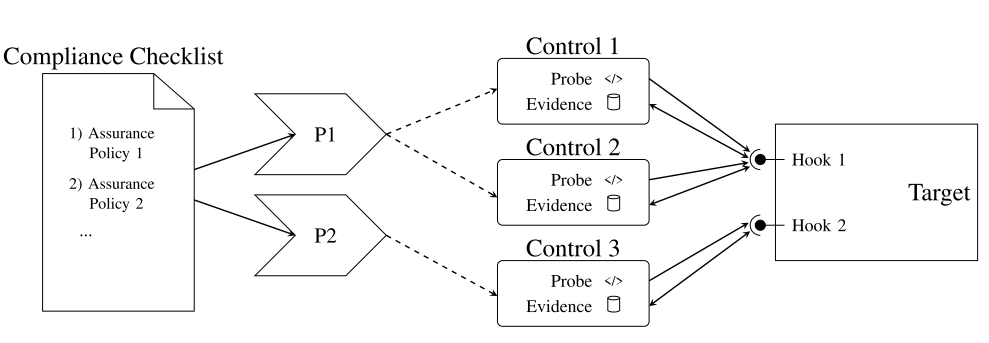
\includegraphics[scale=0.53]{Security_Compliance_Evaluation}
    \caption[Security Compliance Evaluation]{Security Compliance Evaluation}
    \label{fig:Security_Compliance_Evaluation}
\end{figure}
\hfill\break
\break
Moon Cloud implementa il processo di Security Compliance Evaluation in Figura \ref{fig:Security_Compliance_Evaluation} usando Controlli 
di monitoraggio o di test personalizzabili. Inoltre, è dotato delle seguenti caratteristiche, le quali vanno a completare i requisiti 
elencati nella Sezione \ref{list:security-assurance-fondamentals}.
\begin{itemize}
    \item Moon Cloud implementa un sistema di Security Assurance Evidence-based continuo, implementato come processo di Compliance,
    basato su politiche custom o standard; inoltre, presenta una visione olistica dello stato di sicurezza di un dato sistema.
    \item Moon Cloud permette di schedulare e configurare delle ispezioni automatiche, grazie all'inventario di asset protetto e senza
    l'intervento dell'uomo.
    \item Moon Cloud Evaluation Engine può ispezionare dall'interno un sistema, gestendo così delle minaccie interne; permettendo anche 
    reazioni rapide a incidenti di sicurezza e veloci rimedi, grazie alla raccolta continua di evidence.
\end{itemize}
In generale, Moon Cloud gestisce i processi di Evaluation attraverso un set di \textit{Execution Cluster}; ognuno dei quali gestisce 
ed esegue un set di \textit{probe} che collezionano le evidence necessarie per effettuare i processi di valutazione. 
Tutte le attività di collezione sono eseguite dalla probe, ognuno dei quali è uno script Python fornito come una singola immagine di Docker, 
che viene inizializzata quando è triggerata una Evaluation ed è distrutta quando il processo di Evaluation è terminato.\hfill\break
Accedendo alla piattaforma di Moon Cloud, l'utente può definire le proprie politiche di sicurezza e attività di Evaluation come 
una serie di Controlli di sicurezza e altre politiche predefinite. Una volta che una politica viene definita, l'utente può 
decidere quando schedulare l'Evaluation; e nel momento in cui un processo di Evaluation viene inizializzato, tutti i Controlli e/o le 
politiche legate ad essa, vengono eseguiti e i risultati, raccolti dalla probe, vengono memorizzati e restituiti all'utente. 
A questo punto l'utente può accedere a questi risultati a diversi gradi di precisione: una visione sommaria e generale di tutte le 
politche implentate e dello stato generale del sistema di sicurezza, al risultato di una specifica politica oppure alle evidence 
raccolte per una Evaluation.
\vspace{0.5 cm}
\hfill\break
Per poter rendere ancora più intuitivo e semplice da utilizzare un sistema di questa importanza, si è pensato d'introdurre un sistema 
che possa raccomandare agli utenti, in base agli asset che vogliono proteggere e monitorare, una serie di Evaluation o politiche da 
applicare in quei casi; questo permette anche a utenti meno esperti di poter configurare in modo rapido ed efficiente meccanismi di 
protezione da minacce. Un sistema di raccomandazione permette di selezionare all’interno di un ampio catalogo, un numero limitato di prodotti 
personalizzati sulla base delle preferenze dell’utente attivo. La ricerca in questo ambito si è sempre concentrata sulla qualità delle 
raccomandazioni di questi sistemi, tralasciando un aspetto fondamentale: la fiducia che un utente deve avere verso questi ultimi. 
E ciò è ottenibile se si è il più possibile trasparenti nei processi che portano alla nascita dei suggerimenti, partendo da questo 
si può ottenere l'ambita fiducia da parte degli utenti.


% 2- Tecnologie
\chapter{Tecnologie utilizzate}\label{chp:02-technologies}
In questo capitolo sono descritte le tecnologie utilizzate per la realizzazione del progetto unitamente alle motivazioni legate all'uso 
di certi sistemi rispetto ad altri. In particolare viene fornita una panoramica dei sistemi di raccomandazione analizzati e studiati,
nel capitolo successivo vengono approfonditi a livello pratico i sistemi di raccomandazione Memory-based i quali sono stati utilizzati 
per l'implementazione della soluzione.
% SISTEMARE POSIZIONE TABELLA E FOTO DELLA SEZIONE NESTED SET MODEL
%
\section{Perché Python e Django}
\paragraph{Python}
Python è un linguaggio di programmazione ad alto livello, orientato agli oggetti, adatto, tra gli altri usi, a sviluppare applicazioni 
distribuite, scripting, computazione numerica e system testing; ideato e rilasciato pubblicamente per la prima volta nel 1991 dal suo 
creatore Guido van Rossum, programmatore olandese.\hfill\break
Python supporta diversi paradigmi di programmazione, come quello object-oriented (con supporto all'ereditarietà multipla), quello 
imperativo e quello funzionale, e offre una tipizzazione dinamica forte. È fornito di una standard library estremamente ricca, che, 
unitamente alla gestione automatica della memoria e a robusti costrutti per il controllo delle eccezioni, rendono Python uno dei linguaggi 
più ricchi e comodi da usare; inoltre è anche semplice da usare e imparare. 
Python, nelle intenzioni di Guido van Rossum, è nato per essere un linguaggio immediatamente intuibile. La sua sintassi è pulita e snella 
così come i suoi costrutti, decisamente chiari e non ambigui.\hfill\break
Un aspetto inusuale e unico di Python è il metodo che viene usato per delimitare i blocchi di codice.
%
\lstset{style=python_code_style}
\begin{lstlisting}[language=Python, caption={Esempio di programma scritto in Python}]
# Testing if two strings are equals
def test(got, expected):
    if got == expected:
        result = ' OK '
    else:
        result = ' X '
    print('%s got: %s expected: %s' % (result, repr(got), repr(expected)))

def main():
    test('hail', 'hailing')
    test('swiming', 'swimingly')
    test('do', 'do')

if __name__ == '__main__':
    main()
\end{lstlisting}
%
Nei linguaggi come Pascal, C e Perl, i blocchi di codice sono indicati con le parentesi oppure con parole chiave 
(il C e il Perl usano \textbf{{ }}; il Pascal usa \textbf{begin} ed \textbf{end}). In questi linguaggi è solo una convenzione degli sviluppatori il fatto di 
indentare il codice interno ad un blocco, per metterlo in evidenza rispetto al codice circostante. In Python invece di usare parentesi 
o parole chiave, si usa l'indentazione stessa per indicare i blocchi nidificati in congiunzione col carattere "due punti" (:). Si usa 
sia una tabulazione sia un numero arbitrario di spazi, ma lo standard Python è di 4 spazi.
Python è un linguaggio pseudocompilato: un interprete si occupa di analizzare il codice sorgente (semplici file testuali con 
estensione .py) e, se sintatticamente corretto, di eseguirlo, non esiste una fase di compilazione separata (come 
avviene in C, per esempio) che generi un file eseguibile partendo dal sorgente \cite{python-documentation}.
%
\paragraph{Django}
Django è un web framework di alto livello basato su Pyhton che permette di sviluppare rapitamente e con tutti i presupposti per un sistema sicuro, un sito web
perfettamente mantenibile. Esso si occupa della maggiori difficoltà dello sviluppo web, così da permettere di concentrarsi sulla scrittura dell'app; inoltre 
è open-source e ha una comunità attiva, una documentazione completa e semplice da consultare.\hfill\break
Django aiuta a scrivere applicazioni con le seguenti caratteristiche \cite{django-documentation}.
\begin{description}
    \item[Versatile:] può essere usato per la creazione di quasi tutti i tipi di siti web, a partire da sistemi per la gestione di contenuti,
    a social network e siti di notizie; può lavorare con qualunque client-side framework, e gestire contenuti in quasi tutti i formati (inclusi HTML, 
    RSS feeds, JSON, Xml, etc). Internamente permette la scelta e l'implementazione di qualsiasi funzionalità (es. molti dei database più popolari, ecc.).
    \item[Sicuro:] aiuta gli sviluppatori a evitare gli errori più comuni in merito alla sicurezza provvedendo un framework costruito per eseguire 
    le operazioni in modo corretto e sicuro. Ad esempio, Django fornisce un metodo sicuro per gestire gli account degli utenti e le relative 
    password, evitando errori comuni come inserire informazioni riguardanti la sessione dell'utente nei cookies, dove sarebbero vulnerabili (invece i cookie 
    contengono soltanto una chiave, e i valori effettivi sono salvati nel database) o salvare direttamente una password invece di una hash password.
    \item[Mantenibile:] il codice di Django è scritto seguendo i principi e i pattern che incoraggiano la creazione di codice mantenibile e riusabile. Inoltre 
    particolare, fa uso del principio "Don't Repeat Yourself" (DRY) così da ridurre al minimo le duplicazioni non necessarie, diminuendo la quantità di codice.
    Django raggruppa parti di codice letto in moduli seguendo le linee guida del pattern Model View Controller (MVC).
    \item[Portabile:] Django essendo scritto in Python, un linguaggio multi piattaforma, lo rende indipendente dal sistema operativo eseguito sul server, che 
    sia Linux, Windows o Mac OS X. Per di più, Django è ben supportato da molti web hosting provider, che spesso provvedono a specifche infrastrutture
    e documentazione per l'hosting di siti web in Django.
\end{description}
In generale, un tradizionale server web resta in attesa di richieste HTTP da parte del browser web (o altri client) degli utenti; nel momento in cui riceve 
una richiesta (solitamente di tipo POST o GET) 
l'applicazione legge le informazioni contenute in essa, all'interno dell'intestazione e/o del corpo, e nell'URL. A seconda della richiesta è possibile che 
vengano letti o scritti dati da un database o altre operazioni che portino al soddisfacimento della richiesta stessa, a questo punto l'applicazione restituisce una 
risposta al browser web dell'utente che ne ha fatto richiesta, spesso in modo dinamico, creando una pagina HTML, sulla base del Template,
da mostrare, in cui può essere data la possibilità di inserire dati dall'utente in appositi campi compilabili o semplicemente mostrare delle informazioni.
%
\newpage
%
\begin{figure}[ht!]
    \centering
    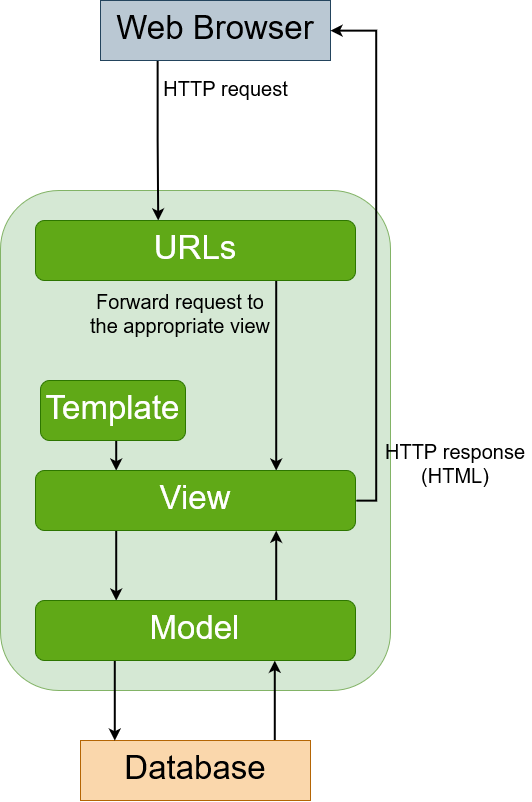
\includegraphics[scale=0.3]{images/Django_doc.png}
    \caption{Schema generico di funzionamento di un applicativo web sviluppato con Django.}
    \label{fig:django_doc}
\end{figure}
\hfill\break
Un'applicazione web in Django tipicamente raggruppa il codice che gestisce questi passaggi in file separati, secondo la 
suddivisione in riquadri verdi della Figura \ref{fig:django_doc} \cite{mdn-django-documentation}, in cui ognuno di questi
gruppi di file svolge delle operazioni ben precise.
\begin{description}
    \item Un \textbf{URL mapper} è usato per reindirizzare le richieste HTTP alla View corretta in base all'URL della richiesta; è possibile processare 
    richieste da qualsiasi URL attraverso una singola funzione, ma è più mantenibile scrivere diverse View per gestire ogni risorsa. 
    Inoltre è possibile controllare se nell'URL è presente un particolare pattern di stringhe o numeri, e passare di conseguenza la richiesta alla 
    funzione appropriata come dati da elaborare.
    \item Una \textbf{View} è una funzione che gestisce le richieste HTTP, e restituisce una risposta HTTP. Le View accedono ai dati necessari per soddisfare la 
    richiesta, anche attraverso i Model, e si delega la formattazione delle risposte ai Template.
    \item I \textbf{Model} sono oggetti in Python che definiscono la struttura dei dati dell'applicazione, e provvedono meccanismi per gestirla (add, modify, 
    delete) e query per interpellare il database.
    \item Un \textbf{Template} è un file di testo che definisce la struttura o il layout di un altro file (come una pagina HTML), attraverso placeholder per
    rappresentare la posizione e il contenuto effettivo. Una View può creare dinamicamente una pagina HTML usando un Template HTML, popolandolo con dati presi dal Model, 
    che a sua volta può recuperli dal database.
\end{description}
Nel Listing \ref{lst:URLex1} si può osservare come viene scritto un URL e come si interfaccia con una View; in questo caso nel 
momento in cui viene fatta una richiesta HTTP a questo URL \textit{recommendation/item/<str:item\_other\_id>/} viene richiamata la 
View \textit{recommendation\_views.item\_recommendation} passando il parametro \textit{<str:item\_other\_id>}.
\lstset{style=python_code_style}
\begin{lstlisting}[language=Python, label=lst:URLex1]
# URL Example 'recommendation/item/35/'
path('recommendation/item/<str:item_other_id>/', recommendation_views.item_recommendation, name='item_recommendation')
\end{lstlisting}
A questo punto, come viene mostrato nel Listing \ref{lst:URLex2}, viene richiamata la View, essa prende i valori che gli vengono passati in ingresso e 
restituisce un risultato, in questo caso viene richiamata la View che implementa il sistema di raccomandazione Item-based, la quale si effettua una ricerca 
nel database per il valore del parametro \textit{<str:item\_other\_id>} in ingresso, verificando l'esistenza di quell'item, questo è possibile
grazie all'ausilio dei Model i quali sono stati utilizzati precedentemente per definire la struttura delle tabelle e dei relativi campi 
contenuti nel database e ora attraverso i cosiddetti QuerySet, messi a disposizione da Django, è possibile accedere a quei dati; successivamente vengono 
determinati tramite l'agoritmo di raccomandazione quali sono i possibili item simili e vengono salvati nella variabile \textit{similar\_item\_evaluations}, 
infine, dopo aver ripulito i dati da informazioni poco rilevanti, viene restiuita una risposta in formato JSON al browser web che ha effettuato la richiesta.
\lstset{style=python_code_style}
\begin{lstlisting}[language=Python, label=lst:URLex2]
# Item recommendation API REST
@api_view(['GET'])
def item_recommendation(request, item_other_id):
    # Trying to retrieve the actual node with item_other_id
    item = Evaluation.objects.get(other_id=item_other_id)

    similar_item_evaluations = item_recommendation_alg(item_other_id)

    # Cleaning the data, deleting all the keys except 'other_id'
    similar_item_evaluations_serilized = EvaluationSerializerRecommendation(similar_item_evaluations, many=True).data

    return JSONResponse(similar_item_evaluations_serilized, safe=False)
\end{lstlisting}
%
\section{Docker}
Docker è una piattaforma software che permette di creare, testare e distribuire applicazioni con la massima rapidità. Docker raccoglie 
le applicazioni in unità standardizzate chiamate \textit{Container} che offrono tutto il necessario per la loro corretta esecuzione, incluse librerie, 
strumenti di sistema, codice e runtime. Con Docker, è possibile distribuire e ricalibrare le risorse per un'applicazione in qualsiasi ambiente, 
tenendo sempre sotto controllo il codice eseguito.\hfill\break
Questa tecnologia utilizza solitamente il kernel di Linux e le sue funzionalità, come Cgroups e namespace, per isolare i processi in modo da poterli 
eseguire in maniera indipendente. Questa indipendenza è l'obbiettivo dei Container: la capacità di eseguire più processi e applicazioni in 
modo separato per sfruttare al meglio l'infrastruttura esistente pur conservando il livello di sicurezza che sarebbe garantito dalla 
presenza di sistemi separati.
%
\begin{figure}[ht!]
    \centering
    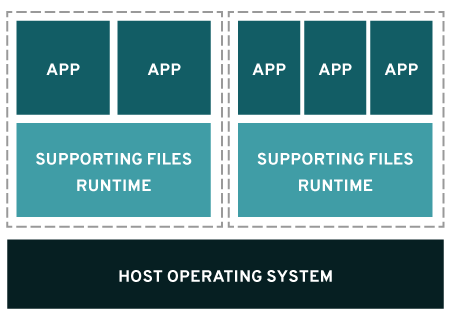
\includegraphics[scale=0.5]{images/Docker_Config_Container.png}
    \caption{Schematizzazione di Container in Docker e di Virtual Machine.}
    \label{fig:DCC}
\end{figure}
\hfill\break
Gli strumenti per la creazione di Container, come Docker, consentono il deployment a partire da un'\textit{immagine}, ciò semplifica la condivisione di 
un'applicazione o di un insieme di servizi, con tutte le loro dipendenze, nei vari ambienti.
Docker, considera i Container come macchine virtuali modulari estremamente leggere, offrendo la flessibilità di creare, distribuire, 
copiare e spostare i Container da un ambiente all'altro, ottimizzando così le app per il cloud.\hfill\break
I Container forniscono una modalità standard per impacchettare il codice delle applicazioni, le configurazioni e le dipendenze, in un singolo oggetto e 
condividono un sistema operativo installato sul server, operando come processi con risorse isolate, assicurando velocità, affidabilità e distribuzioni coerenti, 
indipendentemente dall’ambiente.\hfill\break
%
Questo sistema crea un livello di astrazione fra i Container e il sistema operativo ospitante e gestisce l’attivazione e la disattivazione dei Contenitori. 
Un'altra grande differenza è che la virtualizzazione permette di eseguire più sistemi operativi contemporaneamente in un singolo sistema, mentre i Container 
condividono lo stesso kernel del sistema operativo e isolano i processi applicativi dal resto dell’infrastruttura.
%
\section{Strutture dati gerarchiche}
Nel caso di questa tesi si vogliono memorizzare due tassonomie, aventi struttura ad albero, in cui ogni nodo corrisponde, all'interno di una tabella, ad un 
record; quindi in dati gerarchici si instaurano delle relazioni padre-figlio tra le quali non possono essere rappresentate in modo naturale 
all'interno di un database relazionale, il quale, per l'appunto, segue il Modello Relazionale.\hfill\break
Esso è un modello logico di rappresentazione dei dati all'interno di un database, in cui ogni riga di una tabella è un record identificato univocamente
da una chiave primaria, e le colonne contengono gli attributi dei dati e in genere ogni record ha un valore per ogni attributo.\hfill\break
In questa tesi si è lavorato su un database Sql, in cui i dati normalmente sono conservati come semplici "flat table", e in particolare si è usato il DBMS 
PostgreSQL, un sistema di gestione di database relazionali ad oggetti (ORDBMS). In generale le tabelle contenute in questo tipo di base di dati non permettono la 
memorizzazione secondo un modello gerarchico (come nell'Xml).\hfill\break
Per questo motivo è sorta la necessità di cercare un metodo alternativo per poter rappresentare queste strutture all'interno di database tradizionali.
In questo caso ogni nodo ha un solo padre e nessuno o più figli (a eccezione del nodo radice che non ha un nodo padre); questo genere di rappresentazione 
delle informazioni, può essere trovato in diversi ambiti di applicazione di un database, incluse discussioni su forum e mailing list, 
grafici di organizzazione di un business, categorie per gestire contenuti e prodotti.
%
\begin{figure}[ht!]
    \centering
    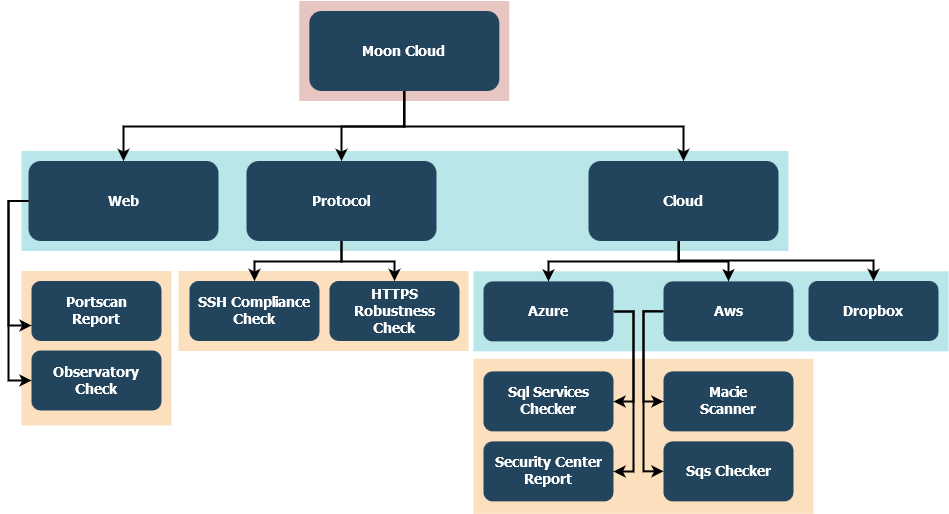
\includegraphics[scale=0.46]{images/MC_Rec_Tree.png}
    \caption{Esempio della rappresentazione gerarchica parziale dei dati nel progetto in questione.}
    \label{fig:MC_Rec_Tree}
\end{figure}
\hfill\break
Durante lo studio compiuto per la realizzazione di questa testi sono stati analizzati diversi approcci per poter gestire le informazioni in modo gerarchico, 
i più importanti presi in considerazione sono i seguenti: 
\begin{itemize}
    \item The Adjacency List Model.
    \item The Nested Set Model.
\end{itemize}
%
\subsection{The Adjacency List Model}
Il primo approccio è chiamato \textit{Adjacency List Model} o metodo ricorsivo; viene definito tale perché il suo funzionamento si basa su una funzione che 
itera per tutto l'albero.\hfill\break
In questo modello, ogni nodo dell'albero contenuto nella tabella ha associato un puntatore al suo nodo padre, e in particolare il nodo radice ha un puntatore 
a un valore NULL per quest'ultimo valore visto che è il nodo di partenza.\hfill\break
La Tabella \ref{table:adjacency_list_model_table} mostra un esempio di possibile rappresentazione parziale dei dati nel database implementato in questo progetto 
secondo questo approccio, utilizzando come riferimento la Figura \ref{fig:MC_Rec_Tree}.
%
\begin{table}[ht!]
\centering
\begin{tabular}[c]{| c | l | c |} 
    \hline
    id & name & parent \\ [0.5ex] 
    \hline
    \rowcolor{rootnodecell} 1 & Moon Cloud & NULL \\ [0.5ex] 
    \rowcolor{categorycell} 2 & Web & 1 \\ [0.5ex] 
    \rowcolor{categorycell} 3 & Protocol & 1 \\ [0.5ex] 
    \rowcolor{categorycell} 4 & Cloud & 1 \\ [0.5ex] 
    \rowcolor{evaluationcell} 5 & Portscan Report & 2 \\ [0.5ex] 
    \rowcolor{evaluationcell} 6 & Observatory Check & 2 \\ [0.5ex] 
    \rowcolor{evaluationcell} 7 & SSH Compliance Check & 3 \\ [0.5ex] 
    \rowcolor{evaluationcell} 8 & HTTPS Robustness Check & 3 \\ [0.5ex] 
    \rowcolor{categorycell} 9 & Azure & 4 \\ [0.5ex] 
    \rowcolor{categorycell} 10 & Aws & 4 \\ [0.5ex] 
    \rowcolor{categorycell} 11 & Dropbox & 4 \\ [0.5ex] 
    \rowcolor{evaluationcell} 12 & Sql Services Checker & 9 \\ [0.5ex] 
    \rowcolor{evaluationcell} 13 & Security Center Report & 9 \\ [0.5ex] 
    \rowcolor{evaluationcell} 14 & Macie Scanner & 10 \\ [0.5ex] 
    \rowcolor{evaluationcell} 15 & Sqs Checker & 10 \\ [0.5ex]
    \hline
\end{tabular}
\caption{Esempio di una possibile tabella per gestire dati in modo gerarchico secondo l'Adjacency List Model.}
\label{table:adjacency_list_model_table}
\end{table}
\hfill\break
Il vantaggio di usare questo modello sta nella sua semplicità di costruzione, soprattutto a livello di codice client-side, 
e di restituzione dei figli di un nodo. Questo approccio diventa problematico nella maggior parte dei linguaggi 
di programmazione perché necessita di una query per ogni nodo dell'albero, e visto che ogni query impiega 
un certo periodo di tempo, questo rende la funzione molto lenta e poco efficiente quando si lavora con alberi di grandi dimensioni. 
Nel Esempio \ref{lst:ex_ALM_query} è possibile osservare come viene recuparata in puro Sql l'intera tassonomia per le Evaluation; 
è possibile notare che la maggiore limitazione di questo approccio è che si necessità di un operazione di JOIN per ogni livello 
della gerarchia, e naturalmente questo porta a un degrado delle performance all'aumentare della complessità; nel caso di questo progetto
si ha una tassonomia a tre livelli, quindi il problema è limitato, ma volendo avere una visione al futuro questo sistema col tempo diventerebbe 
sempre meno performante.
\begin{lstlisting}[language=SQL, label=lst:ex_ALM_query, caption={Query in puro Sql per recuperare l'intera tassonomia delle Evaluation, 
    secondo l'Adjacency List Model.}]
SELECT t1.name AS lev1, t2.name as lev2, t3.name as lev3
    FROM Evaluation AS t1
        LEFT JOIN Evaluation AS t2 ON t2.parent = t1.id
        LEFT JOIN Evaluation AS t3 ON t3.parent = t2.id
    WHERE t1.name = "moon cloud";
\end{lstlisting}
Questa query si può tradurre in codice client-side attraverso una furnzione ricorsiva la quale determina per ogni nodo i suoi figli, per ogni figlio
i suoi figli e così via finchè non si arriva ai nodi foglie.
Inoltre, molti linguaggi non sono ottimizzati per funzioni ricorsive. Per ogni nodo, la funzione crea una nuova istanza di se stessa e 
ogni istanza occupa una porzione di memoria e impiega un certo tempo per inizializzarsi, più grande è l'albero e più questo processo sarà portato a termine 
in maggior tempo.
%
\newpage
%
\subsection{The Nested Set Model}
Il secondo approccio analizzato è il \textit{Nested Set Model}, il quale è stato utilizzato per l'implementazione delle tassonomie per le Evaluation e 
i Controlli (o politiche per verificare il soddisfacimento dei requisiti di sicurezza di un Target o asset indicato dall'utente) all'interno del progetto.\hfill\break
Questo approccio permette di osservare le gerarchie di dati in un modo diverso, non come nodi e linee, come se fosse un albero, ma come container innestati.
%
\begin{figure}[ht!]
    \includegraphics[scale=0.6]{images/MC_Rec_NSM_Container(R).png}
    \caption{Esempio della gestione di dati in modo gerarchico secondo il Nested Set Model, utilizzando quelli presi dal database del 
    progetto in questione (ridotto).}
    \label{fig:MC_Rec_NSM_Container_R}
\end{figure}
%
\hfill\break
%
Con questo sistema la gerarchia viene mantenuta, secondo il principio cui un nodo padre contiene i suoi figli. Questa struttura 
viene mantenuta in tabella attraverso l'uso di due attributi aggiuntivi, \textit{lft} e \textit{rght}, come è possibile osservare 
dalla Tabella \ref{table:nested_set_model_table} seguente, la quale fa riferimento alla Figura \ref{fig:MC_Rec_NSM_Container} 
posta alla fine della sezione.
\begin{table}[ht!]
\centering
\begin{tabular}[c]{| c | l | c | c |}
    \hline
    id & name & lft & rght \\ [0.5ex] 
    \hline
    \rowcolor{rootnodecell} 1 & Moon Cloud & 1 & 100 \\ [0.5ex] 
    \rowcolor{categorycell} 2 & Web & 86 & 99 \\ [0.5ex] 
    \rowcolor{categorycell} 3 & Protocol & 80 & 85 \\ [0.5ex] 
    \rowcolor{categorycell} 4 & Cloud & 4 & 29 \\ [0.5ex] 
    \rowcolor{evaluationcell} 5 & Portscan Report & 91 & 92 \\ [0.5ex] 
    \rowcolor{evaluationcell} 6 & Observatory Check & 89 & 90 \\ [0.5ex] 
    \rowcolor{evaluationcell} 7 & SSH Compliance Check & 83 & 84 \\ [0.5ex] 
    \rowcolor{evaluationcell} 8 & HTTPS Robustness Check & 81 & 82 \\ [0.5ex] 
    \rowcolor{categorycell} 9 & Azure & 13 & 26 \\ [0.5ex] 
    \rowcolor{categorycell} 10 & Aws & 5 & 12 \\ [0.5ex] 
    \rowcolor{categorycell} 11 & Dropbox & 27 & 28 \\ [0.5ex] 
    \rowcolor{evaluationcell} 12 & Sql Services Checker & 22 & 23 \\ [0.5ex] 
    \rowcolor{evaluationcell} 13 & Security Center Report & 20 & 21 \\ [0.5ex] 
    \rowcolor{evaluationcell} 14 & Macie Scanner & 8 & 9 \\ [0.5ex] 
    \rowcolor{evaluationcell} 15 & Sqs Checker & 10 & 11 \\ [0.5ex]
    \hline
\end{tabular}
\caption{Esempio di una tabella per gestire dati in modo gerarchico secondo il Nested Set Model.}
\label{table:nested_set_model_table}
\end{table}
\hfill\break
Dalla Tabella \ref{table:nested_set_model_table} la gerarchia dei dati viene rappresentata attraverso l'uso 
degli attributi \textit{left} e \textit{right} per rappresentare l'annidamento dei nodi (il nome delle colonne: \textit{left} e \textit{right}, hanno significati 
speciali in Sql; per questo motivo si identificano questi campi con i nomi \textit{lft} e \textit{rght}).
%
\newpage
%
\begin{figure}[ht!]
    \centering
    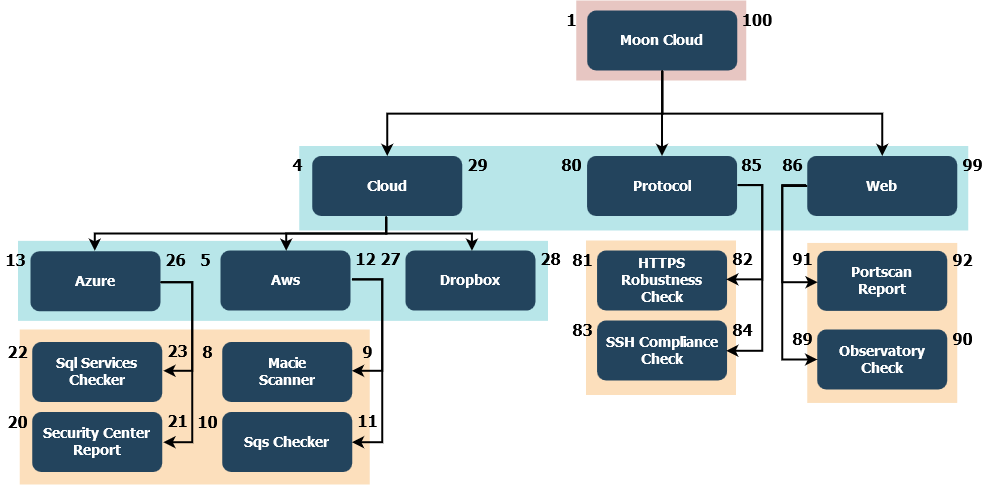
\includegraphics[scale=0.40]{images/MC_Rec_NSM_Tree.png}
    \caption{Esempio della gestione di dati in modo gerarchico secondo il Nested Set Model, utilizzando quelli presi dal database del 
    progetto in questione.}
    \label{fig:MC_Rec_NSM_Tree}
\end{figure}
\vspace{-0.5 cm}
\hfill\break
L'assegnazione di questi valori viene effettuata ad ogni nodo visitandolo due volte e assegnando i valori in ordine di visita, e in entrambe le visite. 
Quindi vengono associati ad ogni nodo due numeri, memorizzati come due attributi. 
Più precisamente si inizia la visita dell'albero partendo da sinistra e continuando verso destra, un livello alla volta, scendendo per ogni 
nodo i suoi figli, assegnando i valori al campo \textit{left}, prima di assegnare un valore al campo \textit{right}, e successivamente si continua verso 
destra. Questo approccio è chiamato \textit{Modified Preorder Tree Traversal Algorithm} (MPTT). A partire da questa tecnica è stato 
ideata la struttura della tassonomia delle evaluation e dei Controlli implementate nella soluzione proposta in questa tesi, con 
l'ausilio di un package di Python chiamato MPTT, del quale verrà illustrato il funzionamento nel capitolo \ref{chp:04-solution}.\hfill\break
Più semplicemente se si osserva la parte superiore della Figura \ref{fig:MC_Rec_NSM_Container_R} si può notare che la numerazione dei nodi, viene 
effettuata a partire da container più esterno da sinistra e continua verso destra.\hfill\break
A prima vista questo approccio può sembrare più complicato da comprendere rispetto all'Adjacency List Model, ma quest'ultimo è 
molto più veloce quando si vuole recuperare i nodi, visto che basta una query, mentre è più lento per operazioni di inserimento e 
cancellazione dei nodi; il Listing \ref{lst:ex_NSM_query} qui di seguito mostra come è possibile recuperare l'itera tassonomia delle Evaluation; si 
può notare che questa query funziona in modo indipendente dalla profondità della tassonomia; inoltre, non è necessario preoccuparsi del valore \textit{rght} 
del nodo all'interno della clausola \textit{BETWEEN} della query perché il valore cadrà sempre all'interno dello stesso nodo padre come anche il 
valore di \textit{lft}.
\begin{lstlisting}[language=SQL, label=lst:ex_NSM_query, caption={Query in puro Sql per recuperare l'intera tassonomia delle Evaluation, 
    secondo il Nested Set Model.}]
SELECT node.name
    FROM Evaluation AS node, Evaluation AS parent
    WHERE node.lft BETWEEN parent.lft AND parent.rgt
        AND parent.name = "moon cloud"
    ORDER BY node.lft;
\end{lstlisting}
Altro esempio è il caso in cui si vuole recuperare tutti i nodi foglia della tassonomia come mostra il Listing \ref{lst:ex_NSM_query2}, in cui è ancora 
più semplice rispetto nell'Adjacency List Model. Nel Nested Set Model, il valori di \textit{lft} e \textit{rght} per i nodi foglia hanno valori 
consecutivi; quindi per trovare i nodi foglia basta cercare quei nodi dove il valore di \textit{rght} è pari a quello di \textit{lft} incrementato di uno.
\begin{lstlisting}[language=SQL, label=lst:ex_NSM_query2, caption={Query in puro Sql per recuperare tutti i nodi foglia della tassonomia delle Evaluation, 
    secondo il Nested Set Model.}]
SELECT name
    FROM Evaluation
    WHERE rgt = lft + 1;
\end{lstlisting}
Infine nel caso di inserimento o cancellazione di un nodo il grado di complessità dell'operazione è determinato dalla posizione del nodo che si 
vuole inserire o cancellare; a partire dal caso più semplice, quando si vuole inserire o cancellare un nodo foglia, quel nodo senza figli, fino 
al caso più complesso, quando si vuole cancellare un nodo padre perchè bisogna anche gestire i suoi nodi figli.
Nel primo caso, è sufficente per poter cancellare un nodo senza figli eseguire una query come mostrata nel Listing \ref{lst:ex_NSM_query3}, si determinano 
prima i valori dei campi \textit{lft} e \textit{rght} e la loro differenza, \textit{width}, successivamente cancellato il nodo si sottrae la sua 
differenza da ogni nodo alla sua destra.
\begin{lstlisting}[language=SQL, label=lst:ex_NSM_query3, caption={Query in puro Sql per eliminare un nodo foglia dalla tassonomia delle Evaluation, 
    secondo il Nested Set Model.}]
SELECT @myLeft := lft, @myRight := rgt, @myWidth := rgt - lft + 1
    FROM Evaluation
    WHERE name = "Sqs Checker";

DELETE FROM Evaluation WHERE lft BETWEEN @myLeft AND @myRight;

UPDATE Evaluation SET rgt = rgt - @myWidth WHERE rgt > @myRight;
UPDATE Evaluation SET lft = lft - @myWidth WHERE lft > @myRight;
\end{lstlisting}
%
Nel secondo caso, in cui voglio eliminare il nodo padre ma non i suoi nodi figli si può decidere che i figli vengano spostati allo stesso livello del 
nodo padre eliminato, ciò viene mostrato dal Listing \ref{lst:ex_NSM_query4}. In questo caso si sottrae due da tutti gli elementi a destra di tale nodo 
(visto che i figli avranno una dimensione, \textit{width}, di due) e uno da tutti i nodi che sono suoi figli (per chiudere il gap creato dalla perdita 
del nodo padre e dal valore associato al campo \textit{lft}).
\begin{lstlisting}[language=SQL, label=lst:ex_NSM_query4, caption={Query in puro Sql per eliminare un nodo padre dalla tassonomia delle Evaluation, 
    secondo il Nested Set Model.}]
SELECT @myLeft := lft, @myRight := rgt, @myWidth := rgt - lft + 1
    FROM Evaluation
    WHERE name = "Web";

DELETE FROM Evaluation WHERE lft = @myLeft;

UPDATE Evaluation SET rgt = rgt - 1, lft = lft - 1 WHERE lft BETWEEN @myLeft AND @myRight;
UPDATE Evaluation SET rgt = rgt - 2 WHERE rgt > @myRight;
UPDATE Evaluation SET lft = lft - 2 WHERE lft > @myRight;
\end{lstlisting}
%
\begin{figure}
    \centering
    \includegraphics[scale=0.56]{images/MC_Rec_NSM_Container.png}
    \caption{Esempio della gestione di dati in modo gerarchico secondo il Nested Set Model, utilizzando quelli presi dal database del 
    progetto in questione.}
    \label{fig:MC_Rec_NSM_Container}
\end{figure}
%
\newpage
%
\section{Sistemi di raccomandazione}
Un sistema di raccomandazione (\textit{Recommendation System}) è un sistema che consiglia a un utente uno o più item esistenti 
presenti in un database; l'\textit{item} è inteso come una qualsiasi cosa di interesse all'utente, come prodotti, libri o giornali. 
Quando si esegue una raccomandazione si ha come obbiettivo quello di consigliare l'item che possa essere tra quelli di maggiore 
interesse; in altre parole, devono essere in accordo con i gusti dell'utente.\hfill\break
Oggigiorno si possono trovare due principali trend di sistemi di raccomandazione.
\begin{description}
    \item[Content-based filtering](CBF): un item viene raccomandato ad un utente se esso è simile ad altri item di interesse o piaciuti 
    in passato, prendendo in considerazione prima gli item con alte valutazioni o quelli molto utilizzati; questo è possibile perché ad 
    ogni item sono associate delle informazioni che lo descrivono, e questo insieme di dati viene definito metadati.
    \item[Collaborative filtering](CF): un item viene raccomandato ad un utente se i suoi vicini (altri utenti simili) sono 
    interessati a quello stesso item.
\end{description}
%
\begin{figure}[ht!]
    \centering
    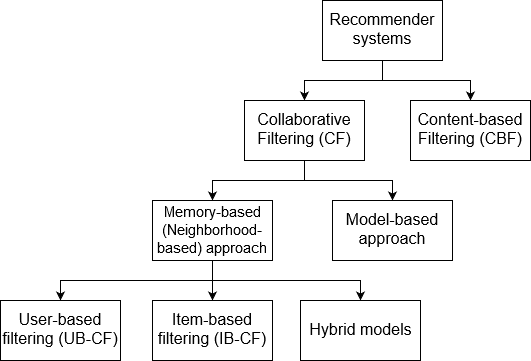
\includegraphics[scale=0.5]{images/recommender_systems.png}
    \caption{Categorizzazione generale dei sistemi di raccomandazione.}
    \label{fig:recommender_systems}
\end{figure}
Entrambi gli approcci hanno i loro punti di forza e di debolezza. Il primo algoritmo si focalizza sul contenuto degli item e
sugli interessi del singolo utente e propone item differenti a utenti differenti, questo significa che ogni utente può ricevere 
raccomandazioni uniche. 
Tuttavia la più grande limitazione del CBF è il fatto di non poter determinare se un utente è interessato ad un item in modo implicito,
perché analizza direttamente i metadati del prodotto e non considera gli interessi di altri utenti, i quali potrebbero 
suggerire item che non verrebbero notati con questo approccio.
Per quanto riguarda il CF, nel caso siano presenti molti contenuti e proprietà associati agli item, allora vengono consumate molte 
risorse e tempo per poter analizzarli, nel contempo a questo algoritmo non interessano queste informazioni. Una raccomandazione 
viene fatta sulla base delle valutazioni degli utenti per gli item, o sugli usi che gli utenti fanno degli item e questo è il suo punto 
di forza perché non si trova a dover analizzare item ricchi di informazioni. Allo stesso tempo è anche il suo punto debole, perché può
portare suggerimenti che potrebbero essere considerati poco adatti sulla base della poca relazione con i profili di alcuni utenti. 
Questo problema è accentuato quando sono presenti nel database molti item che non hanno valutazioni o non sono stati mai usati dagli 
utenti \cite{model-based-approach-for-collaborative-filtering}.
\vspace{0.5 cm}
\hfill\break
Un sistema di raccomandazione filtra i dati usando differenti algoritmi e raccomanda gli item più rilevanti agli utenti attraverso 
un procedimento a 3 fasi.
\begin{description}
    \item[Raccolta di dati:] il primo step è anche quello più importante per poter costruire un sistema di 
    raccomandazione che produca risultanti rilevanti e consistenti. I dati possono essere raccolti in due modi: esplicitamente, 
    cioè attraverso la raccolta diretta di informazioni fornite dagli utenti, ad esempio le valutazioni di un prodotto oppure 
    implicitamente. In questo caso vengono raccolti dati che, non sono prodotti in modo intenzionale dall'utente, ma sono ottenuti 
    dai costanti flussi di dati come la cronologia di ricerca, i click effettuati, lo storico degli ordini, ecc.
    \item[Memorizzazione di dati:] la quantità di dati definisce quanto efficace un modello di raccomandazione possa di 
    diventare. Ad esempio, in un sistema di raccomandazione per film, maggiori sono le valutazioni fornite dagli utenti, e 
    migliore sarà il sistema di raccomandazione per gli altri utenti. Il tipo di dati che si vuole raccogliere determina
    anche il supporto di memorizzazione più adatto.
    \item[Filtraggio dei dati:] dopo la fase di raccolta e memorizzazione dei dati, essi vanno filtrati per poter estrarre 
    le informazioni rilevanti e poter effettuare le raccomandazioni finali, inoltre vi sono diversi algoritmi standard per 
    realizzare quest'ultima fase..
\end{description}
%I sistemi di raccomandazione possono essere suddivisi nelle seguenti categorie, ma spesso si preferisco anche degli approcci ibridi, 
%combinazioni di sistemi di raccomandazione basati sul Contenuto (\textit{Content-based filtering}) e di 
%quelli Collaborativi (\textit{Collaborative filtering}) in modo da essere più efficaci e sfruttare i pregi di entrambi gli approcci.
%
\subsection{Content-based filtering}
Un Content-based filtering (definito anche con l'acronimo CBF) è un sistema di raccomandazione in cui vengono suggeriti, rispetto ad un item, quelli 
più simili, confrontando le informazioni contenute nei metadati, come una descrizione, uno o più autori, la categoria di 
appartenenza, ecc.. L'idea base che si trova dietro questi sistemi, è il fatto che se ad un utente piace o interessa un particolare 
item allora gli piaceranno anche altri con caratteristiche o proprietà simili.\hfill\break
Questo algoritmo suggerisce prodotti che piacevano all'utente nel passato ed è limitato a item dello stesso tipo. Un 
Content-based recommender fa riferimento a quegli approcci che provvedono raccomandazioni comparano la rappresentazione del 
contenuto che descrive un item e la rappresentazione del contenuto dell'item interessato dall'utente.\hfill\break
Questi metodi sono usati quando si conoscono a priori i metadati sugli item che si vuole suggerire, ma nulla sugli utenti.
In questo sistema, delle \textit{keyword} sono utilizzate per caratterizzare gli item e un profilo dell'utente è 
costruito per memorizzare quali item sono di suo interesse. In altre parole, questi algoritmi cercano di raccomandare quello che 
l'utente ha valutato positivamente o usato nel passato e sta esaminando nel presente. La costruzione del profilo dell'utente, 
spesso temporaneo, non viene basata su un modulo di registrazione che l'utente stesso deve compilare, ma su informazioni 
lasciate indirettamente dall'utente, le quali possono essere: i prodotti che ha maggiormente cercato e acquistato, quelli che sono 
stati inseriti nella lista dei desideri, ecc.. Più precisamente, tra vari item candidati da raccomandare all'utente si passa per un 
processo di confronto con gli item piaciuti dall'utente e gli item migliori vengono suggeriti.
%
\subsection{Collaborative filtering}
Il Filtraggio Collaborativo (definito anche con l'acronimo CF) per poter funzionare, si appoggia ad un database che raccoglie le 
preferenze degli utenti sulla base di un insieme di item, che a loro volta possono essere presenti nella stessa base di dati. 
Si sfruttano tecniche di analisi dei dati per poter ottenere delle raccomandazioni che consiglino gli utenti a trovare gli item 
che gli potrebbero piacere,eventualmente producendo una lista dei migliori N item.\hfill\break
Un utente è sottoposto ad un processo di matching per poter scoprire quali sono i possibili \textit{neighbours},
che corrispondono ai possibili utenti aventi storicamente delle preferenze in comune ad egli. Infine, gli item maggiormente 
preferiti dai \textit{neighbours} sono raccomandati all'utente.\hfill\break
Questi sistemi tentano di predire la valutazione o la preferenza che un utente darebbe a un item basandosi sulle preferenze date da altri 
utenti, queste ultime possono essere ottenute o in modo esplicito dagli utenti o tramite misurazioni implicite.
Inoltre i Filtri Collaborativi non richiedono l'uso di metadati associati agli item, come nei Filtri Content-based.\hfill\break
Tuttavia, restano ancora oggi alcune sfide significative a cui sono sottoposti i sistemi di raccomandazione basati su 
Filtraggio Collaborativo.\hfill\break
Il primo obbiettivo è quello di migliorare la scalabilità di questi algoritmi; essi sono in grado di cercare 
anche diecimila potenziali \textit{neighbours} in tempo reale, ma la richiesta dei sistemi moderni è di cercare dieci milioni 
potenziali \textit{neighbours}, per questo motivo possono nascere problemi di performance con i singoli utenti quando essi hanno 
molte informazioni associate.\hfill\break
Il secondo obbiettivo è quello di migliorare la qualità dei sistemi di raccomandazione per gli utenti. Questi ultimi vogliono 
raccomandazioni di cui possono fidarsi e che possono aiutarli a trovare item di loro gusto e interesse.
Per certi versi questi due obbiettivi sono in conflitto tra di loro; per ottenere dei risultati validi e di una certa importanza è 
necessario trattarli in contemporanea perché aumentare solamente la scalabilità diminuirebbe la qualità delle raccomandazioni e viceversa 
\cite{item-based-collaborative-filtering}.\hfill\break
Il principale modello di Filtri Collaborativi studiato in questo elaborato e approfondito nel capitolo successivo, è il metodo definito 
come \textit{Memory-based} e il vantaggio di utilizzare questa tecnica sta nel fatto di essere semplici da implementare e i risultati 
ottenuti sono altrettanto semplici da interpretare; mentre si possono trovare anche Filtri Collaborativi che sfruttano metodi 
\textit{Model-based} che si basano sulla fattorizzazione di matrici e sono molto più funzionali per gestire il problema della 
sparsità dei dati. Questi ultimi sono sviluppati usando algoritmi di data mining e machine learning per predire le valutazioni di utenti 
su item senza valutazioni, tentando di comprimere grandi database in un modello ed effettuare il processo di raccomandazione applicando dei 
meccanismi di riferimento all'interno di questo modello, questo permette ai CF Model-based di rispondere alle richieste degli utenti 
istantaneamente \cite{model-based-approach-for-collaborative-filtering}.
%
\subsection{Il problema della Cold Start}
Cosa succederebbe se un nuovo utente o un nuovo item venisse aggiunto al database? Questa situazione è chiamata \textit{Cold Start} ed 
è possibile trovarne di due tipi.
\begin{description}
    \item[Visitor Cold Start:] si verifica quando un nuovo utente viene aggiunto al database, e visto che non è presente alcuno storico relativo, 
    il sistema non è a conoscenza delle sue preferenze; per questo motivo diventa molto più difficile raccomandare prodotti a quel particolare utente. 
    Per risolvere questo problema, a livello teorico, si potrebbe applicare un procedimento di raccomandazione basata sulla popolarità dei prodotti, ma solo una 
    volta che si è venuti a conoscenza delle preferenze dell'utente, sarà possibile generare delle raccomandazioni più precise e adeguate alle sue esigenze.
    \item[Item Cold Start:] si verifica quando un nuovo item viene inserito nel sistema. L'azione dell'utente è quella più importante per determinare 
    il valore di questo item all'interno dell'ecosistema; quindi maggiore è l'interazione che un item riceve maggiore è la facilità che venga raccomandato 
    all'utente interessato.
\end{description}


% 3- Recommendation systems
\chapter{Collaborative filtering}
\label{chp:03-recommendationSystems}
In questo capitolo verranno approfonditi gli algoritmi di raccomandazione implementati nella soluzione, mostrando le porzioni di 
codice e spiegando i vari passagi che portano ad ottenere delle raccomandazioni.
% - nel capitolo dei recommendation system parlare dei collaborative filter in modo più dettagliato e legato al progetto -


\section{Memory-based} 
I Filtri Collaborativi Memory-based sono stati introdotti per via delle osservazioni che vennero fatte dalla comunità, dicenddo che
gli utenti si fidano maggiormente delle raccomandazioni di altri che la pensano allo stesso modo. Questi metodi mirano a calcolare 
le relazioni tra utenti e item attraverso lo schema dei vicini che identifica sia coppie di item che tendono ad essere usati insieme 
o hanno un grado di similarità alto o utenti con uno storico di item usati simile. \cite{taxonomy-of-recommender-agents-on-the-internet}
Questi approcci divennero molto famosi grazie alla loro semplicità di implementazione, molto intuitivi, non necessitano di operazioni
di training sui dati e regolazione di molti parametri, inoltre l'utente può capire la ragione che sta dietro ogni raccomandazione. 

Questa categoria di sistemi di raccomandazione sono definiti anche \\\textit{Neighborhood-based} e possono essere ulteriormente classificati 
in due sottocategorie:


\subsection{User-based filtering} 
Questo sistema, definiti anche con l'acronimo UB-CF (\textit{User-based Collaborative Filter}) basa tutto il suo funzionamento sulla 
comunità di utenti, maggiore è la sua dimensione e l'attività degli utenti con item o servizi e migliori potranno essere le 
raccomandazioni. Questo algoritmo fornisce dei suggerimenti ad un utente sulla base di uno o più vicini, e la similarità tra utenti può
essere determinata sulla base degli item che l'utente ha utilizzato o valutato.

Molti di questi approcci possono essere generalizzati dall'algoritmo organizzato nei seguenti passi:
\begin{enumerate}
	\item Specificare qual'è l'utente a cui si vuole applicare l'algoritmo di raccomandazione e recuperare quali utenti possono 
	avere dato valutazioni o usato item simili al utente target. Piuttosto che recuperare tutti gli utenti, per velocizzare l'esecuzione
	dell'algoritmo, è possibile selezionare soltanto un gruppo di utenti in modo casuale oppure associare dei valori di similarità tra 
	tutti gli utenti e confrontando questi valori con quello dell'utente target, selezionare i relativi utenti che superano una soglia
	scelta, oppure utilizzare tecniche di clustering.
	\item Estrarre quegli item a cui l'utente target non ha mai interagito e per questo motivo gli possono interessare, e mostrarli 
	sottoforma di raccomandazioni.
\end{enumerate}

\begin{figure}[ht!]
	\centering
	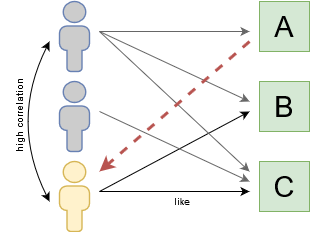
\includegraphics[scale=0.5]{images/UB_CF_ex.png}
	\caption{Esempio di applicazione di un sistema di raccomandazione User-based}
	\label{fig:UB_CF}
\end{figure}

Questi approcci sono facilmente implementabili, indipendenti dal contesto in cui sono applicati e possono essere più accurati rispetto
a tecniche basate sul Content-based filtering; dall'altra parte all'aumentare del numero di utenti che vado a considerare per fare le 
raccomandazioni migliore è la precisione di questo processo ma anche è maggiore il costo in termini di tempo.  

Nella soluzione proposta in questa tesi, l'algoritmo UB-CF viene implentato come funzione che prende in ingresso un parametro 
(\textit{user\_other\_id}), come è possibile osservare da \ref{lst:UB_CF_1} corrispondente all'identificativo per l'utente, 
e restituisce una lista di raccomandazioni (\textit{similar\_user\_evaluations}) corrispondenti alle Evaluation simili a quelle usate 
da altri utenti. 

\lstset{style=python_code_style}
\begin{lstlisting}[language=Python, label=lst:UB_CF_1]
# User recommendation algortihm
def user_recommendation_alg(user_other_id):
\end{lstlisting}
\ \\
Più precisamente il funzionamento dell'algoritmo si svolge seguendo i seguenti passi:
\begin{itemize}
	\item il primo passo è quello di recuperare sulla base del parametro in ingresso alla funzione, lo user\_other\_id,
	tutte le Evaluation che l'utente in questione ha utilizzato;
	\begin{lstlisting}[language=Python, label=lst:UB_CF_2]
		# Select the target user and its evaluations
		target_user_evaluations = User.objects.get(other_id=user_other_id).evaluations.all()\
																					.values('other_id', 'id', 'parent_id')\
																					.order_by('other_id')
	\end{lstlisting}
	\item il secondo passo consiste nel selezionare le Evaluation usate dagli altri utenti, e viene create una lista di queste Evaluation;
	\begin{lstlisting}[language=Python, label=lst:UB_CF_3]
		# Select all other users and theirs evaluations
		other_users = User.objects.exclude(other_id=user_other_id)
		# Creating a list with all the evaluations of other users
		other_users_evaluations = []
		for o_users_evaluation in other_users:
			for evaluation in o_users_evaluation.evaluations.all().values('other_id', 'id', 'parent_id')\
																	.order_by('other_id'):
				other_users_evaluations.append(evaluation)
	\end{lstlisting}
	\item il terzo passo consiste nell'andare a determinare quali tra le Evaluation dell'utente a cui si vuole raccomandare quali sono quelle 
	simili usate dagli altri utenti. Per determinare le Evaluation simili si è andato a confrontare il paramentro \textit{parent\_id} (identifica
	all'interno della tassonomia quale sia il nodo padre per quella Evaluation), associato ad ogni Evaluation, in questo modo si è andati a selezionare
	soltanto gli item appartenenti a una stessa categoria, eliminando eventuali nodi duplicati. E componendo una lista finale con le Evaluation
	restanti.
	\begin{lstlisting}[language=Python, label=lst:UB_CF_4]
		# Comparing target user's evaluations and other user's evaluations, and if there is a match the evaluation is
		# added to the 'similar_evaluations' list (the matching is made comparing the 'parent_id')
		similar_user_evaluations = []
		for t_user_evaluation in target_user_evaluations:
			for o_users_evaluation in other_users_evaluations:
				# Taking only the evaluations that have: different other_id (excluding the target evaluation
				# in the recommendation) and same parent_id and the evaluations that weren't added to 'target_user_evaluations'
				# list and to 'similar_user_evaluations'
				if ((t_user_evaluation['other_id'] != o_users_evaluation['other_id']) and  # Evaluations must have different 'other_id'
						(t_user_evaluation['parent_id'] == o_users_evaluation['parent_id']) and  # Evaluations must have the same 'parent_id'
						# Evaluation in all_other_evals list mustn't be already added to \
						not (o_users_evaluation in target_user_evaluations) and  # the 'target_user_evaluations' list or
						not (o_users_evaluation in similar_user_evaluations)):  # the 'similar_user_evaluations' list
					similar_user_evaluations.append(o_users_evaluation)
	\end{lstlisting}
\end{itemize}

%% ESEMPIO DI UNA CHIAMATA CON VALORE DI RITORNO
%\begin{figure}[ht!]
%	\centering
%	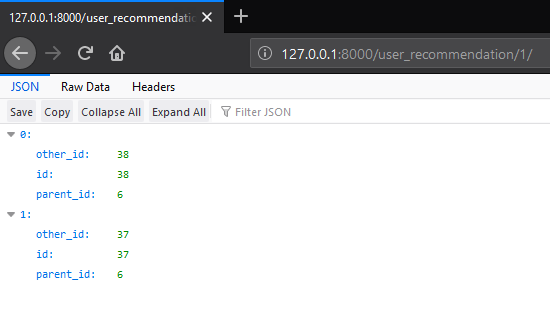
\includegraphics[scale=0.5]{images/UB_CF_test.png}
%	\caption{Esempio di esempio di una risposta in JSON a una chiamata Rest all'algoritmo di raccomandazione UB-CF.}
%	\label{fig:UB_CF_resp_json}
%\end{figure}
\ \\
Nel capitolo successivo verrano mostrati degli esempio pratici in cui è stato applicato questo algoritmo.

\newpage

\subsection{Item-based filtering} 
Quando viene applicato per milioni di utenti e item, l'algoritmo UB-CF non è molto efficente, per via della complessa computazione della 
ricerca di utenti simili; così in alternativa è stato introdotto l'algoritmo di filtraggio Item-based, definito anche IB-CF 
(\textit{Item-based Collaborative Filter}) dove piuttosto che effetuare il confronto tra utenti simili, viene fatto un confronto tra 
gli item dell'utente a cui si vuole raccomandare e i possibili item simili.

\begin{figure}[ht!]
	\centering
	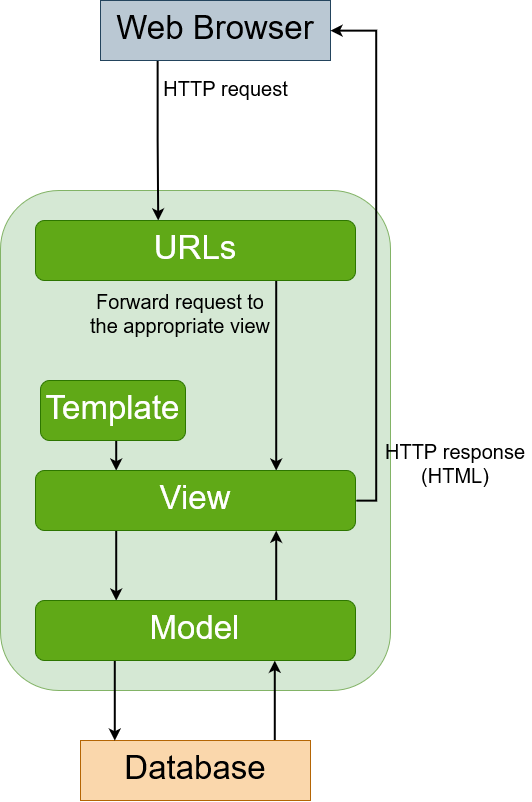
\includegraphics[scale=0.5]{images/IB_CF_ex.png}
	\caption{Esempio di applicazione di un sistema di raccomandazione IB-CF.}
	\label{fig:IB_CF}
\end{figure}
\ \\
Questi sistemi sono estremamente simili ai sistemi di raccomandazione Content-based, e identificano item simili in base a come utenti gli
hanno usati nel passato \cite{item-based-collaborative-filtering}.

A livello pratico nella soluzione proposta, questo algoritmo è stato implementato come funzione che prende in ingresso un 
parametro item\_other\_id rappresentante l'other\_id, un attributo associato ad ogni nodo della tassonomia che lo identifica,
del item su cui si vuole ottenere altri item simili; in generale per determinare la similarità tra due oggetti, si osserva 
l'attributo parent\_id associato ad ogni item, che determina quale sia il nodo padre all'interno della tassonomia, quindi alla fine 
vengono selezionati quegli item che appartengono alla stessa categoria.\\

In generale CF-IB ideato per determinare Evaluation simili funziona seguendo i seguenti passi:
\begin{itemize}
	\item il primo passo è quello di recuperare sulla base del parametro in ingresso alla funzione, lo item\_other\_id,
	l'Evaluation su cui si vuole determinare le altre Evaluation simili;
	\begin{lstlisting}[language=Python, label=lst:IB_CF_Evaluation_1]
	def item_recommendation_alg(item_other_id):

		# Selecting the evaluation, which is applied this algorithm, from its other_id
		# SELECT * FROM recommendation_app_evaluation WHERE other_id = %(item_other_id)s AND node_type = 'eva'
		target_eval = Evaluation.objects.filter(Q(other_id=item_other_id) & Q(node_type="eva"))\
										.values('other_id', 'id', 'parent_id')[0]
	\end{lstlisting} 
	\item il secondo passo è quello di recuperare tutte le Evaluation, escludendo la prima recuperata, presenti nella base di dati;
	\begin{lstlisting}[language=Python, label=lst:IB_CF_Evaluation_2]
		# Selecting the other evaluations, excluding the target evaluation
		# SELECT * FROM recommendation_app_evaluation WHERE other_id != %(item_other_id)s AND node_type = 'eva'
		all_other_evals = Evaluation.objects.filter(~Q(other_id=item_other_id) & Q(node_type="eva"))\
											.values('other_id', 'id', 'parent_id').order_by('other_id')
	\end{lstlisting}
	\item il terzo ed ultimo passo consiste nel andare a determinare le Evaluation che hanno lo stesso parent\_id, quindi
	quelle appartenenti alla stessa categoria, dell'Evaluation ottenuta nel primo passo; inoltre, se presenti, vengono 
	eliminati eventuali duplicati;
	\begin{lstlisting}[language=Python, label=lst:IB_CF_Evaluation_3]
		# Creating a list with all the evaluations that are similar to the target evaluation (comparing the parent_id)
		similar_item_evaluations = []
		for evaluation in all_other_evals:
			# Taking only the evaluations that have: different other_id (excluding the target evaluation
			# in the recommendation) and same parent_id and the evaluations that weren't added to similar_item_evaluations
			# list
			if ((target_eval['other_id'] != evaluation['other_id']) and  # Evaluations must have different 'other_id'
					(target_eval['parent_id'] == evaluation['parent_id']) and  # Evaluations must have same 'parent_id'
					# Evaluation in all_other_evals list mustn't be already added to \
					not (evaluation in similar_item_evaluations)): # the 'similar_item_evaluations' list
				similar_item_evaluations.append(evaluation)

	return similar_item_evaluations	
	\end{lstlisting}
\end{itemize}

%% ESEMPIO DI UNA CHIAMATA
%\begin{figure}[ht!]
%	\centering
%	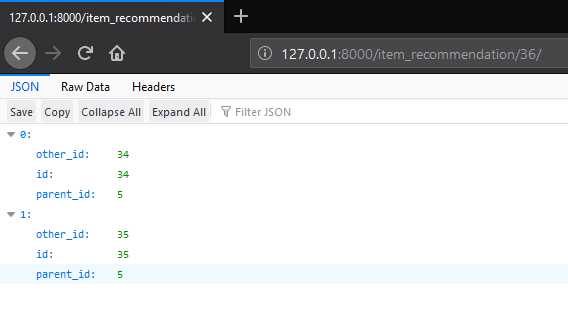
\includegraphics[scale=0.5]{images/IB_CF_Evaluation_test.png}
%	\caption{Esempio di esempio di una risposta in JSON a una chiamata Rest all'algoritmo di raccomandazione IB-CF per le Evaluation
%	supportate da Moon Cloud.}
%	\label{fig:IB_CF_Eval_resp_json}
%\end{figure}

Altro algoritmo del tipo IB-CF implementato in questa tesi sulla falsa riga di quello appena riportato qua sopra, è quello ideato per
determinare quali Evaluation possono essere raccomandate per un Target inserito da un utente tra quelli supportati da Moon Cloud,
che sono: Host avente Windows come sistema operativo, Host avente Linux come sistema operativo, sistemi che sfruttano 
servizi di Aws o di Azure e Url di siti web. \\
In Python questo algoritmo viene implementato come funzione che prende in ingresso l'id (identificativo univoco) del Target, e 
restituisce l'insieme delle Evaluation raccomandate per quel Target, il tutto viene eseguito seguendo questi passi:
\begin{itemize}
	\item il primo passo è quello di recuperare tutte le Evaluation presenti nel database;
	\begin{lstlisting}[language=Python, label=lst:IB_CF_Target_1]
	def target_recommendation_alg(target_id):
		# Retriving all the evaluations in the database
		evaluations = Evaluation.objects.filter(node_type="eva")
	\end{lstlisting} 
	\item il secondo ed ultimo passo è quello di andare a determinare quali sono i Controlli che hanno lo stesso target\_type\_id
	del Target id passato come parametro della funzione, e da quei Controlli determinare le Evaluation che li utilizzano, 
	eliminando eventuali duplicati; determinando così le possibili Evaluation applicabili per quel Target.
	\begin{lstlisting}[language=Python, label=lst:IB_CF_Target_2]
		# Saving in the target_evaluations list the evaluations which controls have target_type_id equal to target_id
		target_evaluations = []
		for evaluation in evaluations: # Scanning all the evaluations
			for evaluation_controls in evaluation.controls.filter(target_type_id=target_id):
				if not(evaluation in target_evaluations): # Excluding evaluations duplicated
					target_evaluations.append(evaluation)
	
		# Converting the Evaluation model's instance in a dict and putting the evaluation, as a dict, in a list
		target_evaluations_serializer = EvaluationSerializer(target_evaluations, many=True)

		return target_evaluations_serializer.data
	\end{lstlisting} 
\end{itemize}

%% ESEMPIO DI UNA CHIAMATA
%\begin{figure}[ht!]
%	\centering
%	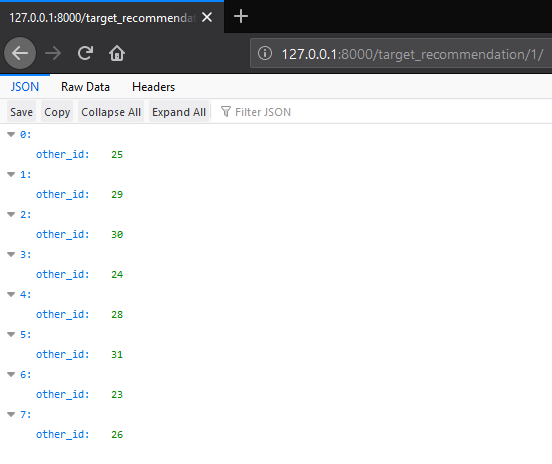
\includegraphics[scale=0.5]{images/IB_CF_Target_test.png}
%	\caption{Esempio di esempio di una risposta in JSON a una chiamata Rest all'algoritmo di raccomandazione IB-CF per i 
%	Target supportarti da Moon Cloud.}
%	\label{fig:IB_CF_Target_resp_json}
%\end{figure}

Nel capitolo successivo verrano mostrati anche degli esempi dei valori di risposta di queste funzioni.

\subsection{Hybrid filtering} 
Nei sistemi di raccomandazione ibridi si tende a voler combinare più tecniche di raccomandazione, cercando di raggruppare i 
pregi di ciascuna tecnica; infatti se uno compara i sistemi di raccomandazione ibridi con i sistemi Collaborativi o 
Content-based, la precisione dei suggerimenti è solitamente maggiore.\\

Nella soluzione proposta in questa tesi, questo algoritmo viene direttamente implementato come Api Rest, alla quale viene 
passato come parametri la request, l'oggetto HTTP che il browser invia al server contenente la richiesta HTTP attraverso
un certo URL e lo user\_other\_id è un valore che viene preso dall'URL, e rappresenta l'other\_id dell'utente su cui si andrà
a raccomandare. Inoltre il tutto viene limitato ad essere richiamato solo tramite richieste HTTP con metodo GET.\\ 
Nel codice \ref{lst:CF_Hybrid_Evaluation_1} possiamo vedere come vengono limitate le richieste al metodo GET e come 
viene definita la funzione.

\begin{lstlisting}[language=Python, label=lst:CF_Hybrid_Evaluation_1, caption={\ }]
@api_view(['GET'])
def hybrid_recommendation(request, user_other_id)
\end{lstlisting} 

Il funzionamento di questo algoritmo si svolge nei seguenti passi:
\begin{itemize}
	\item il primo passo è quello di verificare se l'utente esiste nel database altrimenti viene generata un eccezione (errore) che viene gestito in
	modo personalizzato, generando una risposta HTTP con codice di errore 404 (Not Found);
	\begin{lstlisting}[language=Python, label=lst:CF_Hybrid_Evaluation_2]
		# Trying to retrive the actual User with user_other_id
		user = User.objects.get(other_id=user_other_id)
	\end{lstlisting} 
	\item il secondo passo è applicare l'algoritmo di User Recommandation, descritto nella sezione precendete, per le Evaluation e ottenere due liste,
	la prima target\_user\_evaluations contiene le Evaluation che l'utente ha utilizzato, mentre nella seconda similar\_user\_evaluations si avranno
	le Evaluation che gli altri utenti hanno utilizzato e che sono simili alle Evaluation del primo utente;
	\begin{lstlisting}[language=Python, label=lst:CF_Hybrid_Evaluation_3]
		# Taking from the user_recommendation_alg the evaluation recommended from this approach (similar_user_evaluations)
		# and the user's evaluations (target_user_evaluations)
		target_user_evaluations, similar_user_evaluations = user_recommendation_alg(user_other_id)
	\end{lstlisting} 
	\item il terzo passo consiste nell'applicazione dell'algoritmo Item-based per ogni Evaluation usata dall'utente in questione così da ottenere 
	delle raccomandazioni che sono compatibili con le Evaluation usate dall'Utente; la similarità o appartenenza alla stessa categoria viene 
	ottenuta osservando il valore del parent\_id; anche in questo caso vengono eliminati eventuali duplicati e viene formata una lista 
	similar\_item\_evaluations contenente le Evaluation simili ottenute dall'applicazione dell'algoritmo di raccomandazione Item-based;
	\begin{lstlisting}[language=Python, label=lst:CF_Hybrid_Evaluation_4]
		# For every evaluation used by users is extracted all other possible evaluations that have the same 'parent_id'
		similar_item_evaluations = []
		for t_user_evaluation in target_user_evaluations:  # for every target user's evaluations
			for item_evaluation in item_recommendation_alg(t_user_evaluation['other_id']):  # is applied the item_recommendation algorithm
				# Taking only the evaluations that have: different other_id (excluding the target evaluation
				# in the recommendation) and same parent_id and the evaluations that weren't added to 'similar_item_evaluations'
				# list or to 'similar_user_evaluations' or to 'target_user_evaluations'
				if ((t_user_evaluation['other_id'] != item_evaluation['other_id']) and # Evaluations must have different 'id'
						(t_user_evaluation['parent_id'] == item_evaluation['parent_id']) and # Evaluations must have the same 'parent_id'
						# Evaluation in all_other_evals list mustn't be already added to \
						not (item_evaluation in similar_item_evaluations) and # the 'similar_item_evaluations' list,
						not (item_evaluation in similar_user_evaluations) and # the 'similar_user_evaluations' list or
						not (item_evaluation in target_user_evaluations)): # the 'target_user_evaluations' list
					similar_item_evaluations.append(item_evaluation)
	\end{lstlisting} 
	\item il quarto passo consiste nel raggruppare le due liste contenenti le Evaluation raccomandate per l'utente secondo l'applicazione dei
	due algoritmi, eliminando anche eventuali duplicati, così da ottenere un'unica lista similar\_evaluations la quale viene ritornata dalla 
	funzione sottoforma di risposta HTTP in formato Json;
	\begin{lstlisting}[language=Python, label=lst:CF_Hybrid_Evaluation_5]
		# Putting together the evaluations recommended in similar_user_evaluations list and similar_item_evaluations list
		similar_evaluations = []
		# Adding to similar_evaluations list the evaluation in the similar_user_evaluations list
		for s_user_evaluation in similar_user_evaluations:
			similar_evaluations.append(s_user_evaluation)
		# Adding to similar_evaluations list the evaluation in the similar_item_evaluations list
		for item_evaluation in similar_item_evaluations:
			# Taking only the evaluations that weren't added to \
			if (not (item_evaluation in similar_evaluations) and # the 'similar_evaluations' list or
					not (item_evaluation in target_user_evaluations)): # the 'target_user_evaluations' list
				similar_evaluations.append(item_evaluation)
		similar_evaluations = sorted(similar_evaluations, key=lambda i: i['other_id'])

		return JsonResponse(similar_evaluations, safe=False)
	\end{lstlisting} 
\end{itemize}
\ \\
Nel capitolo successivo verrà mostrato un esempio di risposta quando viene chiamata questa funzione, e verrà approfondito il contesto che 
è stato costruito attorno agli algoritmi di raccomandazione descritti in questo capitolo.

%% ESEMPIO DI UNA CHIAMATA
%\begin{figure}[ht!]
%	\centering
%	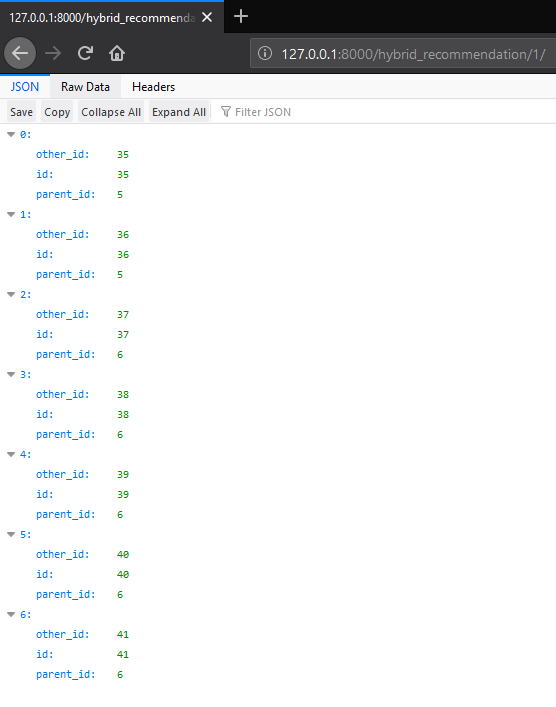
\includegraphics[scale=0.5]{images/CF_Hybrid_test.png}
%	\caption{Esempio di esempio di una risposta in JSON a una chiamata Rest all'algoritmo di raccomandazione Ibrido.}
%	\label{fig:CF_Hybrid_resp_json}
%\end{figure}

% 4- Descrizione del mio progetto
\chapter{Descrizione della soluzione}\label{chp:04-solution}
In questo capitolo è approfondito l'aspetto puramente pratico e le fasi che hanno portato alla realizzazione della soluzione; 
inoltre vengono mostrate le applicazioni pratiche degli aspetti teorici enunciati nei capitoli precedenti, unitamente alle difficoltà 
principali incontrate.
%\vspace{1.5 cm}
%\hfill\break
\section*{Preparazione della base di dati}
Prima di poter costruire il sistema di raccomandazione proposto in questa tesi, sono state eseguite delle operazioni preliminari 
per poter impostare il progetto di Django e la relativa applicazione che implementerà effettivamente la soluzione.
%
% TASSONOMIE E DATABASE CON I MODELS (package MPTT)
Come annunciato nei capitoli precedenti per procedere alla costruzione di un sistema di raccomandazione bisogna avere a disposizione 
una base di dati solida da cui attingere tutte le informazioni; ed è proprio questo il primo passo che è stato seguito, disegnare 
e progettare un database da cui partire per la realizzazione degli algoritmi proposti.
In generale Moon Cloud possiede una struttura delle Evaluation e dei Control ad albero, di conseguenza anche le tabelle del database 
rispecchiano questa struttura, partendo dalle considerazioni fatte sulle tecniche descritte nei capitoli precedenti si è deciso, che 
per implementare un database relazionale che gestisse dati gerarchici, di utilizzare la tecnica
definita come \textit{Modified Preorder Tree Traversal Algorithm}, la quale permette di massimizzare l'efficienza nelle 
operazioni di recupero dei dati, e quindi velocizzare i processi di raccomandazione, ma scendendo a compromessi per quanto riguarda le 
operazioni di inserimento e spostamento dei nodi all'interno della struttura. 
Grazie al package MPTT, il quale è una app di Django che ha come obbiettivo semplificare il più possibile la realizzazione dei 
Model, utilizzati per la generazione della base di dati, e la 
gestione della struttura di dati ad albero; si prende cura di tutti i dettagli riguardanti la realizzazione delle tabelle e dei 
campi \textit{left} e \textit{right} associati ad ogni nodo della tassonomia, e vengono messi a disposizione dei tool per poter 
lavorare con le istanze dei Model. Qui di seguito nel Listing \ref{lst:model} è possibile trovare le porzioni principali del codice 
costituenti i Model.
%
% MODELS CODES
\lstset{style=python_code_style}
\begin{lstlisting}[language=Python, label=lst:model, caption={Parti principali del codice dei Models della soluzione.}]
# TARGET TYPE MODEL

class TargetType(models.Model):
    """
    Target supported by Moon Cloud system
    """
    TYPES = (
        ('host', 'host'),
        ('windows', 'windows'),
        ('url', 'url'),
        ('azure', 'azure'),
        ('aws', 'aws')
    )
    name = models.CharField(max_length=150, choices=TYPES, default="host")
    descr = models.TextField(max_length=1000, default="none")  # Description of a target

    def __str__(self):
        return str(self.name)

    class Meta:
        ordering = ["id"]


# CONTROL MODEL

class Control(MPTTModel):
    """
    Controls that can be part of Evaluations
    """
    other_id = models.IntegerField(default=-1, unique=True)
    parent = TreeForeignKey('self', on_delete=models.CASCADE, null=True, blank=True, related_name='children')
    name = models.CharField(max_length=150, unique=True)
    descr = models.TextField(max_length=1000, default="none")  # Description of a node in the taxonomy
    TYPES = (
        ('cat', 'category'),
        ('con', 'control')
    )
    # Possible node type of the taxonomy (category node or control node)
    node_type = models.CharField(max_length=3, choices=TYPES, default='cat')
    target_type = models.ForeignKey(TargetType, blank=True, null=True, on_delete=models.CASCADE)  # It's null for the root node and category nodes

    def __str__(self):
        return str(self.name)

    class MPTTMeta:
        level_attr = 'level'
        order_insertion_by = ['name']

    class Meta:
        ordering = ['tree_id', 'lft']


# EVALUATION MODEL

class Evaluation(MPTTModel):
    """
    Evaluation is composed by one or more Controls, and can be used by Users
    """
    other_id = models.IntegerField(default=-1, unique=True)
    parent = TreeForeignKey('self', on_delete=models.CASCADE, null=True, blank=True, related_name='children')
    name = models.CharField(max_length=150, unique=True)
    descr = models.TextField(max_length=1000, default="none")  # Description of a node in the taxonomy
    TYPES = (
        ('cat', 'category'),
        ('eva', 'evaluation')
    )
    # Possible node types of the taxonomy (category node or evaluation node)
    node_type = models.CharField(max_length=3, choices=TYPES, default='cat')
    controls = models.ManyToManyField(Control)  # Evaluation can be composed of one or more controls

    def __str__(self):
        return str(self.name)

    class MPTTMeta:
        level_attr = 'level'
        order_insertion_by = ['name']

    class Meta:
        ordering = ['tree_id', 'lft']


# USER MODEL

class User(models.Model):
    """
    User registered to MoonCloud with an email address, and can insert Target and launch Evaluations
    """
    other_id = models.IntegerField(default=-1, unique=True)
    email = models.EmailField(max_length=50, unique=True)
    evaluations = models.ManyToManyField(Evaluation, blank=True)  # Evaluations chosen by user

    def __str__(self):
        return str(self.email)

    class Meta:
        ordering = ["other_id", "id"]


# TARGET MODEL

class Target(models.Model):
    """
    Target (can be more than one) chosen by the user
    """
    user = models.ForeignKey(User, on_delete=models.CASCADE)  # User has chosen a target_type
    other_id = models.IntegerField(default=-1, unique=True)
    target_type = models.ForeignKey(TargetType, on_delete=models.CASCADE)  # TargetType Id

    def __str__(self):
        return str(self.user) + " " + str(self.other_id) + " " + str(self.target_type)

    class Meta:
        ordering = ["user"]
\end{lstlisting}
%
A partire da questi Model vennero introdotte nel database le seguenti tabelle, le quali è possibile visionare nella Figura 
\ref{fig:str_db_project}.
\begin{description}
    \item[Control:] è contenuto l'insieme dei software, o soltanto i riferimenti, che vengono poi effettivamente eseguiti all'interno 
    di una Evaluation, i campi other\_id (identificativo dell'Evaluation che fa riferimento al database effettivo di Moon Cloud), 
    descr (una descrizione del funzionamento del controllo), node\_type (definisce se il nodo è un Evaluation o un nodo Categoria) 
    definiscono le caratteristiche del controllo mentre lft, rght, tree\_id, level e parent sono introdotti 
    automaticamente dal package MPTT per poter rappresentare i dati in modo gerarchico, infine target\_type\_id rappresenta, quel 
    controllo a quale Target viene associato.
    \item[Evaluation:] è contenuto l'insieme di Evaluation che un utente può eseguire per un certo Target, e allo stesso modo 
    i campi contenuti nella tabella Control. La tabella intermedia evaluation\_controls permette di memorizzare quali Controlli 
    sono associati a quali Evaluation.
    \item[User:] sono contenuti gli utenti registrati alla piattaforma Moon Cloud, e sono anche loro, come con le tabelle precedenti, 
    identificati con un campo other\_id, e distinti da un email. La tabella intermedia user\_evaluations permette di memorizzare 
    quali Evaluation un utente ha selezionato e usato.
    \item[Target:] è utilizzata per memorizzare quali Target (o asset) un utente ha inserito e sui quali vuole effettuare dei processi 
    di monitoraggio e verifica, attraverso l'applicazione di politiche e Evaluation.
    \item[TargetType:] vengono specificati quali sono i tipi di Target supportati da Moon Cloud. In generale sono supportati: \textit{Url}, 
    rappresentante l'Url dell'applicativo web, \textit{Host}, viene specificato l'indirizzo Ip identificativo di un host e viene fatta una 
    distizione tra sistema operativo \textit{Windows} o \textit{Linux} eseguito su esso, \textit{Aws}, rappresentante il servizio di cloud computing del 
    gruppo Amazon, e \textit{Azure}, definisce un servizio cloud fornito da Microsoft.
\end{description}
\begin{figure}
    \centering
    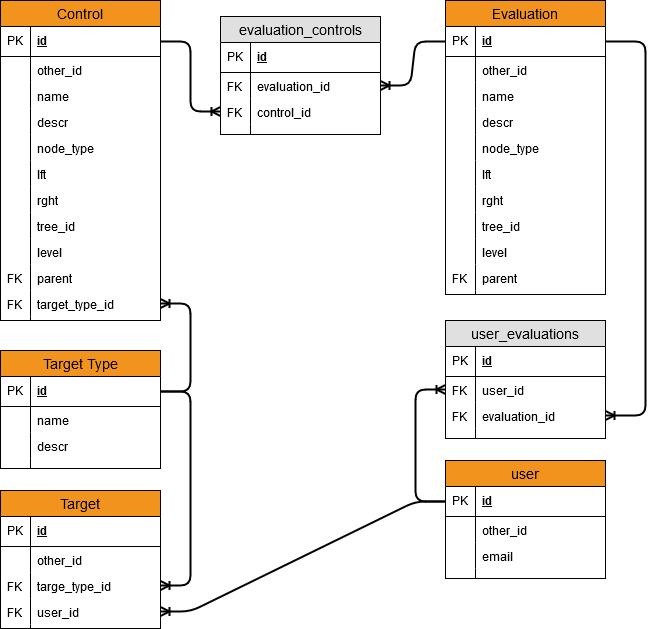
\includegraphics[scale=0.6]{images/MoonCloudRecommendation_ER.png}
    \caption{Struttura del database.}
    \label{fig:str_db_project}
\end{figure}
%
\newpage
%
% VIEW A SCOPO DIDATTICO
%\hfill\break
\section*{Realizzazione delle View}
Successivamente per poter testare che la tassonomia creata per le Evalution e i Controlli fosse corretta e funzionante si è 
implementata un'interfaccia Web a scopo didattico.
Avviando il server, la home page che viene proposta è mostrata nella Figura \ref{fig:MCRS_homepage}, e subito 
sotto è possible trovare il Listing \ref{lst:view_homepage}, dalla quale è possibile 
accedere alle pagine specifiche per la navigazione della tassonomia delle Evaluation piuttosto che dei Controlli; inoltre 
tramite la barra di navigazione è possibile tornare a questa home page o accedere alla admin page generata da Django, e 
succesivamente personalizzata, per poter manipolare la base di dati, e aggiungere, eliminare item o utenti.
%
\begin{figure}[ht!]
    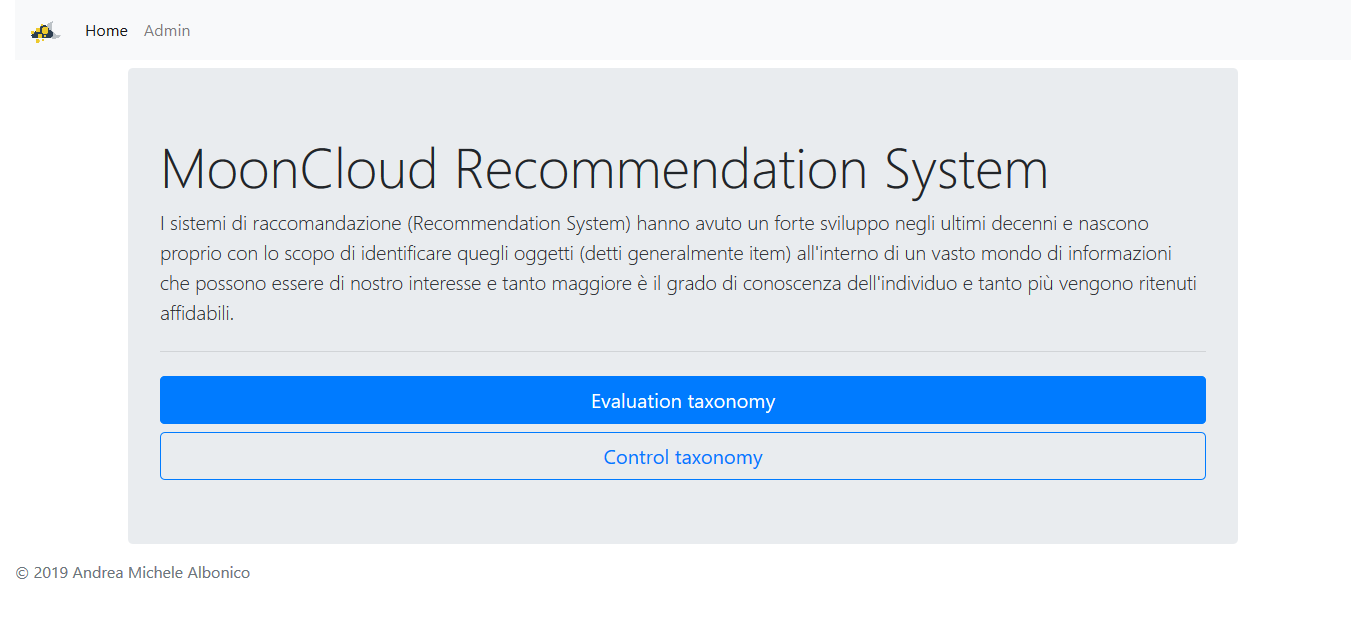
\includegraphics[scale=0.3]{images/MCRS_homepage.png}
    \caption{Home page.}
    \label{fig:MCRS_homepage}
\end{figure}
\lstset{style=python_code_style}
\begin{lstlisting}[language=Python, label=lst:view_homepage, caption={Parte principale del codice delle View della soluzione per gestire l'accesso 
    alla home page.}]
def index(request):
    """
    Index page where you can choose to navigate the evaluation taxonomy or the control taxonomy.
    :param request: HTTP request
    :return: HTTP response with the template to show to the user
    """
    return render(request, "recommendation_app/index.html")
\end{lstlisting}
%
Una volta scelta la tassonomia, di Controlli o delle Evaluation, su cui si vuole navigare, è possibile svolgere diverse attività. 
Dalla Figura \ref{fig:MCRS_taxindex} è possibile osservare l'interfaccia dalla quale si eseguono le operazioni di seguito descritte, e
immediatamente sotto al Listing \ref{lst:view_tax_homepage} è visibile il codice che implementa questa pagina web.\hfill\break
%
\begin{figure}[ht!]
    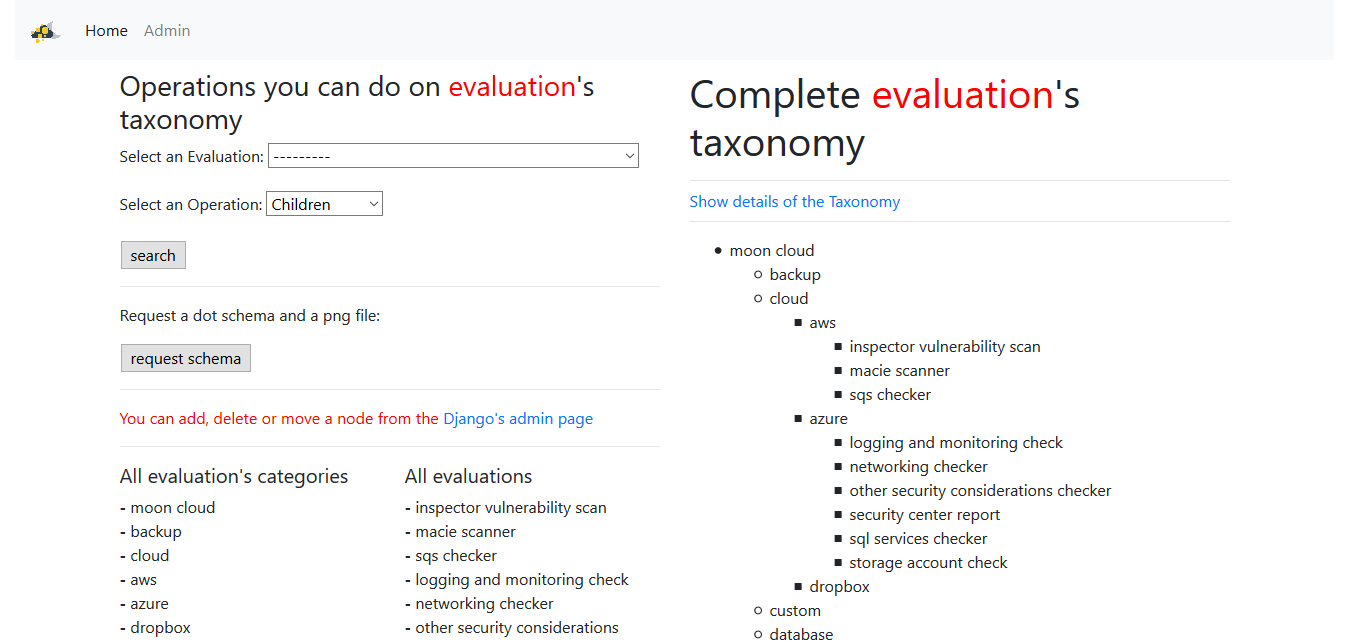
\includegraphics[scale=0.3]{images/MCRS_taxindex.png}
    \caption{Home page per la navigazione della tassonomia.}
    \label{fig:MCRS_taxindex}
\end{figure}
%
\lstset{style=python_code_style}
\begin{lstlisting}[language=Python, label=lst:view_tax_homepage, caption={Home page dalla quale è possibile richiamare 
    diverse operazioni svolgibili sulla tassonomia.}]
def tax_index(request, taxonomy_used):
    """
    The home page shows all taxonomy and a form to make operations on it.
    :param request: HTTP request
    :param taxonomy_used: specify if it's used the Control taxonomy or the Evaluation taxonomy
    :return: HTTP response with the template to show to the user
    """
    # If this is a POST request we need to process the form data
    if request.method == 'POST':
        # Create a form instance and populate it with data from depending on the taxonomy_used
        if (taxonomy_used == "evaluation"):
            form = EvaluationOperationForm(request.POST)
        else:
            form = ControlEvaluationForm(request.POST)
        # Check whether it's valid:
        if form.is_valid():
            # Process the data in form.cleaned_data as required
            nodename_form = form.cleaned_data['nodeName']
            taxonomy_operation_form = form.cleaned_data['actionTax']
            # Redirect to a new URL (page that show a part of the taxonomy, depending on the action user has chosen):
            return redirect(
                reverse('rec:tax_index', args=[taxonomy_used]) + str(nodename_form) + '_' + taxonomy_operation_form)
    # If id's a GET method we'll create a blank form
    else:
        if (taxonomy_used == "evaluation"):
            form = EvaluationOperationForm()
        else:
            form = ControlEvaluationForm()

    # Depending on the taxonomy_used, I'm getting all the categories of Evaluations or Controls taxonomy and save it in a
    # list called "categories_list"
    if (taxonomy_used == "evaluation"):
        q_categories = Evaluation.objects.filter(node_type='cat')
    else:
        q_categories = Control.objects.filter(node_type='cat')
    categories_list = []
    for node in q_categories:
        categories_list.append(node.name)

    # Depending on the taxonomy_used, I'm getting all the categories of Evaluations or Controls node in the taxonomy
    # and save it in a list called "node_list"
    if (taxonomy_used == "evaluation"):
        q_nodes = Evaluation.objects.filter(node_type='eva')
    else:
        q_nodes = Control.objects.filter(node_type='con')
    node_list = []
    for node in q_nodes:
        node_list.append(node.name)

    # Depending on the taxonomy_used, I'm getting all the Evaluations or Controls taxonomy
    if (taxonomy_used == "evaluation"):
        tax = Evaluation.objects.all()
    else:
        tax = Control.objects.all()

    # Passing the complete taxonomy and data to fill the form so you can operate on the taxonomy
    args = {'tax': tax,
            'categories': categories_list,
            'nodes': node_list,
            'form': form,
            'request_path': taxonomy_used}

    return render(request, "recommendation_app/tax_index.html", args)
\end{lstlisting}
%
Le attività che è possibile svolgere sulla tassonomia, sia dei Controlli sia delle Evaluation, sono i seguenti, mentre le operazioni 
di manipolazione dei dati memorizzati dalla base di dati vengono svolte con l'ausilo della admin page messa a disposizione da Django.\hfill\break
\begin{itemize}
    \item Per ogni singolo nodo è possibile recuperare: i discendenti, i figli, la famiglia o i fratelli. Si ottiene un risultato come nella
    Figura \ref{fig:MCRS_taxnodedetails} nel caso in cui si è scelti l'Evaluation Http robustness check e si vuole ritornare tutta label
    famiglia di quel nodo.
    %
    \begin{figure}[ht!]
        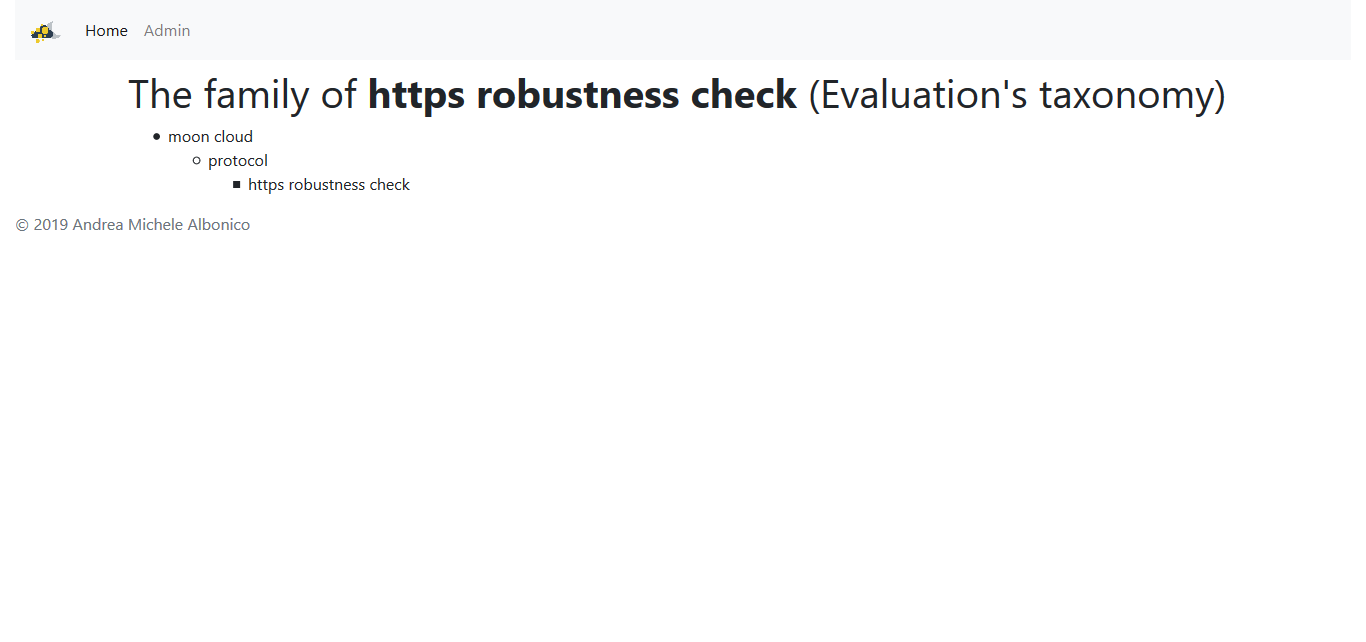
\includegraphics[scale=0.3]{images/MCRS_taxnodedetails.png}
        \caption{Risultato dell'operazione selezionata sul nodo in questione.}
        \label{fig:MCRS_taxnodedetails}
    \end{figure}
    %
    \lstset{style=python_code_style}
    \begin{lstlisting}[language=Python, label=lst:view_tax_nodedetails, caption={Codice utilizzato all'interno delle View per 
        implementare le operazioni per restituire i discendenti, i figli, la famiglia o i fratelli.}]
    # Methods to navigate the taxonomy

    def show_descendants(request, nodename, taxonomy_used):
        """
        Based on the MPTT's method 'get descendants' that return the descendants of a model instance, in tree order
        :param request: HTTP request
        :param nodename: name (it's unique for each node) of a node in the taxonomy
        :param taxonomy_used: specify if it's used the Control taxonomy or the Evaluation taxonomy
        :return: HTTP response with the template to show to the user
        """
        if (taxonomy_used == 'evaluation'):
            q_result = Evaluation.objects.get(name=nodename).get_descendants(include_self=False)
            # Get the count of descendants of the model instance
            q_result_num = Evaluation.objects.get(name=nodename).get_descendant_count()
        else:
            q_result = Control.objects.get(name=nodename).get_descendants(include_self=False)
            # Get the count of descendants of the model instance
            q_result_num = Control.objects.get(name=nodename).get_descendant_count()

        return render(request, "recommendation_app/tax_node_details.html",
                    {'tax_type': (str(taxonomy_used)).capitalize(),
                    'descendants': q_result,
                    'node_exe': nodename,
                    'method': 'descendants',
                    'num_descendants': q_result_num})


    def show_children(request, nodename, taxonomy_used):
        """
        Based on the MPTT's method 'get children' that return the immediate children of a model instance, in tree order
        :param request: HTTP request
        :param nodename: name (it's unique for each node) of a node in the taxonomy
        :param taxonomy_used: specify if it's used the Control taxonomy or the Evaluation taxonomy
        :return: HTTP response with the template to show to the user
        """
        if (taxonomy_used == 'evaluation'):
            q_result = Evaluation.objects.get(name=nodename).get_children()
        else:
            q_result = Control.objects.get(name=nodename).get_children()

        return render(request, "recommendation_app/tax_node_details.html",
                    {'tax_type': (str(taxonomy_used)).capitalize(),
                    'children': q_result,
                    'node_exe': nodename,
                    'method': 'children'})


    def show_family(request, nodename, taxonomy_used):
        """
        Based on the MPTT's method 'get family' that return the ancestors, the model instance itself and the descendants,
        in tree order
        :param request: HTTP request
        :param nodename: name (it's unique for each node) of a node in the taxonomy
        :param taxonomy_used: specify if it's used the Control taxonomy or the Evaluation taxonomy
        :return: HTTP response with the template to show to the user
        """
        if (taxonomy_used == 'evaluation'):
            q_result = Evaluation.objects.get(name=nodename).get_family()
        else:
            q_result = Control.objects.get(name=nodename).get_family()

        return render(request, "recommendation_app/tax_node_details.html",
                    {'tax_type': (str(taxonomy_used)).capitalize(),
                    'family': q_result,
                    'node_exe': nodename,
                    'method': 'family'})


    def show_siblings(request, nodename, taxonomy_used):
        """
        Based on the MPTT's method 'get siblings' that return siblings of the model instance (root nodes are considered
        to be siblings of other root nodes)
        :param request: HTTP request
        :param nodename: name (it's unique for each node) of a node in the taxonomy
        :param taxonomy_used: specify if it's used the Control taxonomy or the Evaluation taxonomy
        :return: HTTP response with the template to show to the user
        """
        if (taxonomy_used == 'evaluation'):
            q_result = Evaluation.objects.get(name=nodename).get_siblings()
        else:
            q_result = Control.objects.get(name=nodename).get_siblings()

        return render(request, "recommendation_app/tax_node_details.html",
                    {'tax_type': (str(taxonomy_used)).capitalize(),
                    'siblings': q_result,
                    'node_exe': nodename,
                    'method': 'siblings'})
    \end{lstlisting}
    \item Attraverso il pulsante \textit{request schema} nella home page della tassonomia si può effetuare una richiesta di stampa in formato .png e del 
    relativo file scritto in notazione DOT rappresentante la tassonomia stesso sotto forma di albero, che contiene i relativi dati salvati all'interno 
    della base di dati.\hfill\break
    Il DOT è un linguaggio descrittivo per grafi, tipicamente i file hanno estensione .gv o .dot, che in combinazione con il software Graphivz è possibile 
    effetuare il rendere della sintassi dot in un immagine più significativa. Qui di seguito nel Listing \ref{lst:DOT_eval} viene mostrato un esempio di 
    scrittura con linguaggio DOT.
    \lstset{style=python_code_style}
    \begin{lstlisting}[language=Python, label=lst:DOT_eval, caption={Codice parziale utilizzato per realizzare lo schema della tassonomia
        per le Evaluation.}]
    graph {
        1 [label="moon cloud"]
        12 [label="protocol"]
        1 -- 12
        11 [label="infrastructure"]
        1 -- 11
        4 [label="cloud"]
        1 -- 4
        16 [label="backup"]
        1 -- 16
        2 [label="database"]
        1 -- 2
        13 [label="web"]
        1 -- 13
        9 [label="human"]
        1 -- 9
        8 [label="custom"]
        1 -- 8
        3 [label="operating system"]
    }
    \end{lstlisting}
    %
    \lstset{style=python_code_style}
    \begin{lstlisting}[language=Python, label=lst:view_DOT_eval, caption={Codice utilizzato per la realizzazione del
        file .dot e relativa immagine .png.}]
    def dot_graph(request, taxonomy_used):
        """
        Create the .dot file (based on the Dot language) and the graph showing the taxonomy in .png format
        :param request: HTTP request
        :param taxonomy_used: specify if it's used the Control taxonomy or the Evaluation taxonomy
        :return: HTTP response with the template to show to the user
        """
        # Create a graph object
        taxonomy_dot_object = Graph(comment='Taxonomy', format='png')
        # Fill the graph with every node in the database (evaluations/controls node and categories nodes), 
        # and create a link with the parent node
        if (taxonomy_used == 'evaluation'):
            taxonomy_nodes = Evaluation.objects.all()
        else:
            taxonomy_nodes = Control.objects.all()
        i = 0
        for node in taxonomy_nodes.order_by('level'):
            # This If construct will prevent the adding of an empty node to the root node in the graph
            if (i == 0):
                # Insert the root node
                taxonomy_dot_object.node(str(node.id), label=str(node.name))
            else:
                # Insert the other nodes
                taxonomy_dot_object.node(str(node.id), label=str(node.name))
                taxonomy_dot_object.edge(str(node.parent_id), str(node.id))
            i += 1
        # Specify where I want to save the .png image and the .dot file
        taxonomy_dot_object.render('taxonomy_output/taxonomy.dot')

        # This function is used to zip a directory
        def make_zipdir(path, ziph):
            # Ziph is zipfile handle
            for root, dirs, files in os.walk(path):
                for file in files:
                    ziph.write(os.path.join(root, file))

        # Making the zip file
        zip_file = zipfile.ZipFile('taxonomy_output.zip', 'w', compression=zipfile.ZIP_DEFLATED)
        make_zipdir('taxonomy_output/', zip_file)
        zip_file.close()

        # Remove the directory which was zipped and all files inside
        shutil.rmtree("taxonomy_output/")

        return redirect(reverse('rec:index'))
    \end{lstlisting}
    \item Inoltre è possibile osservare in maniera più approfondita le informazioni rilevanti sulla tassonomia contenute nelle 
    tabelle del database; e nel caso, della tassonomia delle Evaluation, è possibile simulare il processo di Item Recommendation, 
    premendo il relativo tasto al nodo su cui si vuole determinare le altre Evaluation simili.
    %
    \begin{figure}[ht!]
        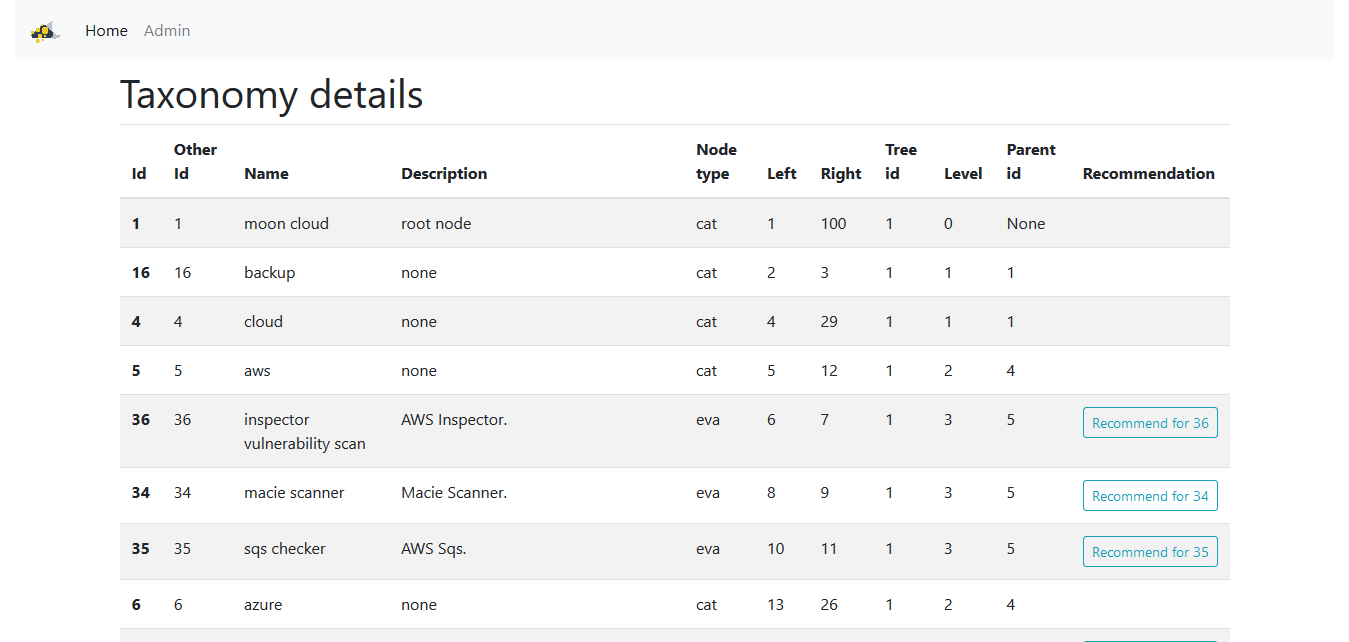
\includegraphics[scale=0.3]{images/MCRS_taxdetails.png}
        \caption{Dettagli della tassonomia sotto forma di tabella come nella base di dati.}
        \label{fig:MCRS_taxdetails}
    \end{figure}
    %
    \lstset{style=python_code_style}
    \begin{lstlisting}[language=Python, label=lst:view_taxdetails, caption={Codice utilizzato per la realizzazione della View che 
        implementa la pagina web del dettaglio della Tassonomia.}]
    def tax_details(request, taxonomy_used):
        """
        Show the taxonomy's details page showing an overview of the taxonomy
        :param request: HTTP request
        :param taxonomy_used: specify if it's used the Control taxonomy or the Evaluation taxonomy
        :return: HTTP response with the template to show to the user
        """
        if (taxonomy_used == 'evaluation'):
            tax_details_obj = Evaluation.objects.all()
        else:
            tax_details_obj = Control.objects.all()

        return render(request, "recommendation_app/tax_details.html",
                    {'tax_details': tax_details_obj,
                    'taxonomy_used': taxonomy_used})
    \end{lstlisting}
\end{itemize}
%
% --------------------------------------------------------------------------------------------------------------------
%\newpage
%
% ASPETTI DI DJANGO CHE HO PERSONALIZZATO, COME LE ADMIN PAGE
Per poter agilmente manipolare la base di dati, Django mette a disposizione la cosiddetta Admin Page mostrata in 
Figura \ref{fig:MCRS_adminpage}, che è stata personalizzata per mostrare le tabelle su cui è possibile 
effetuare modifiche, e per ognuna vengono mostrate le informazioni più rilevanti, come mostrato dalla 
Figura \ref{fig:MCRS_adminpage_evaluationEX} nel caso della tabella Evaluation, e dalla quale è possibile 
effetuare ricerche, eliminare direttamente i dati contenuti nel database e aggiungere 
nuovi dati, come mostrato in Figura \ref{fig:MCRS_adminpage_evaluationEX_add}.
%
\begin{figure}
    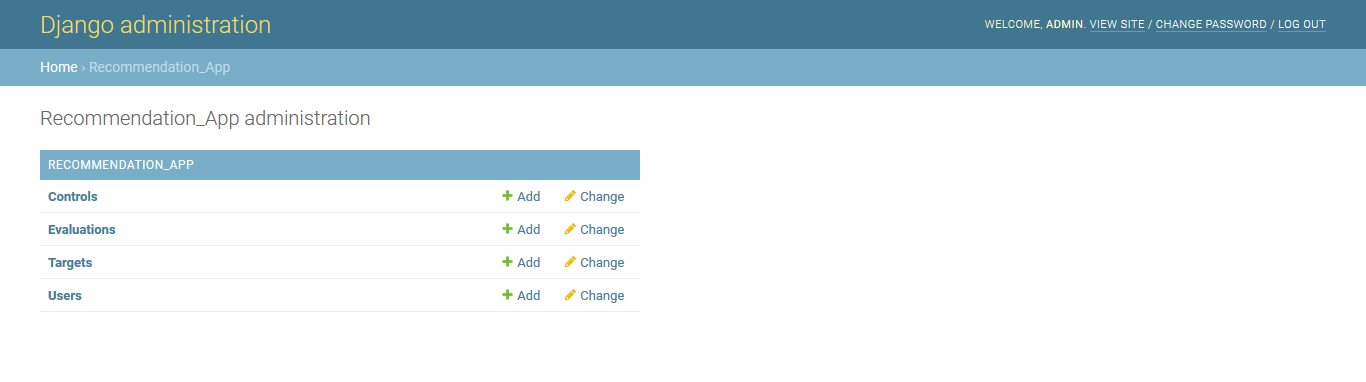
\includegraphics[scale=0.3]{images/MCRS_adminpage.png}
    \caption{Admin page.}
    \label{fig:MCRS_adminpage}
\end{figure}
%
\begin{figure}
    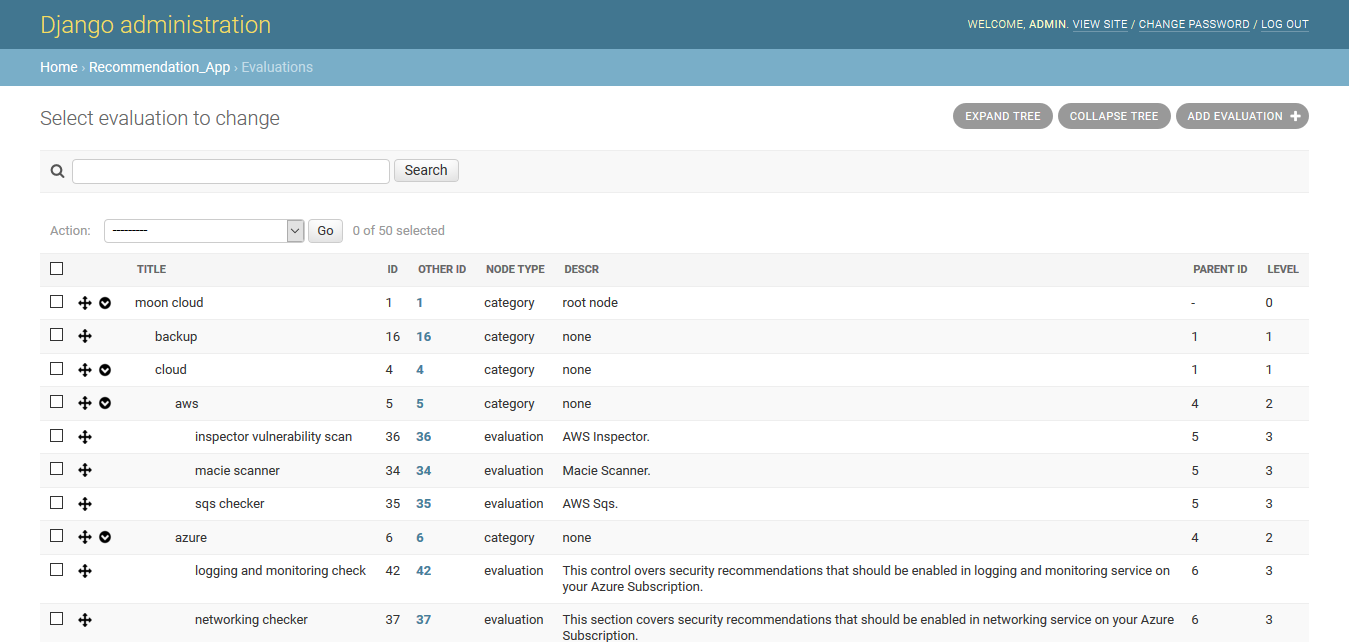
\includegraphics[scale=0.3]{images/MCRS_adminpage_evaluationEX.png}
    \caption{Esempio di Admin page per le Evaluation.}
    \label{fig:MCRS_adminpage_evaluationEX}
\end{figure}
%
\begin{figure}
    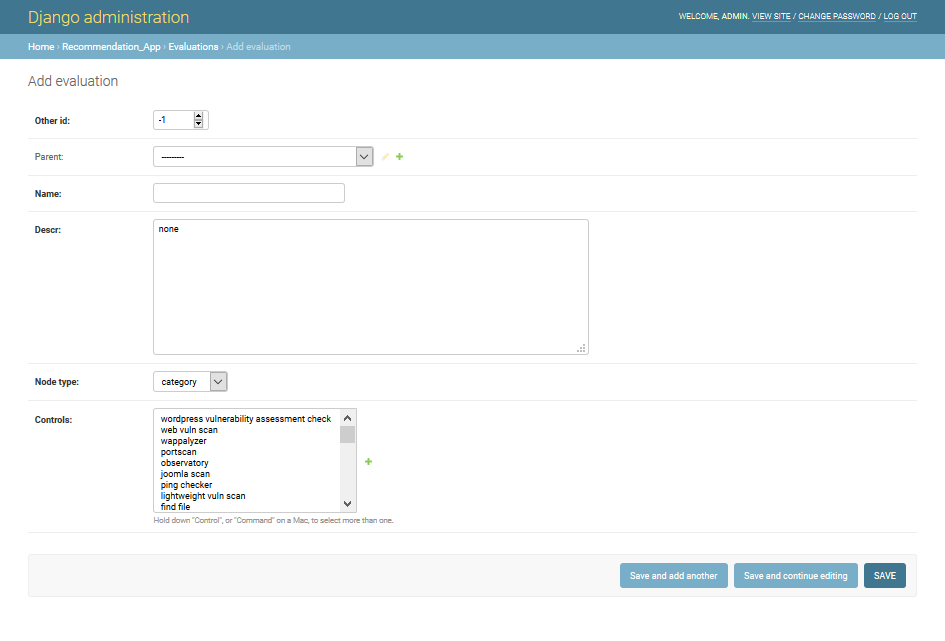
\includegraphics[scale=0.55]{images/MCRS_adminpage_evaluationEX_add.png}
    \caption{Esempio di Admin page per il caso in cui si vuole aggiungere una nuova Evaluation.}
    \label{fig:MCRS_adminpage_evaluationEX_add}
\end{figure}

% VIEW PER LE RACCOMANDAZIONI
\section*{View per i processi di raccomandazione}
%METTO ANCHE DEGLI ESEMPI

% VIEW PER MANTERE LA CONSISTENZA COL MIO DATABASE
\section*{Consistenza tra i database}

% IMPLEMENTAZIONE CON DOCKER
\section*{Implementazione in Docker}

% Documentazione con Postman e parlo dei test

% 5- Conclusioni
\chapter{Conclusioni}\label{chp:05-conclusion}
La soluzione proposta in questa tesi vuole introdurre un sistema di raccomandazione in un mondo in cui spesso non vengono 
introdotti perché popolato da utenti esperti che non ne avrebbero bisogno; invece con il progetto qui proposto si darebbe una
possibilità a un maggior numero di utenti di accedere a servizi su un sistema Cloud di Security Assurance, come 
Moon Cloud, in totale sicurezza e affidabilità.\hfill\break
Con questo lavoro è stato possibile studiare e approfondire il linguaggio di programmazione Python, unitamente al framework 
Django per la realizzazione di applicativi web e la tecnologia Docker per il rilascio in ambienti isolati e indipendenti 
di software; inoltre sono stati approfonditi i temi legati ai Recommendation System e al mondo del machine learning.
%
\section{Sviluppi futuri}
Il sistema di raccomandazione sviluppato in questo tesi offre delle raccomandazioni di tipo basico, tuttavia è in grado di 
supportare gli utenti nell'utilizzo della piattaforma Moon Cloud. Offre altresì spunti di miglioramento, ad esempio 
l'introduzione di un sistema di valutazione delle Evaluation o dei Controlli da parte dell'utente così da incrementare 
la precisione del sistema di raccomandazione, il quale terrebbe conto anche di queste valutazioni.




%       CHIUSURA DELLA TESI     %
\backmatter

% Bibliografia
\printbibliography[heading=bibintoc, title={Bibliografia}]

\end{document}
